% !TeX program = pdflatex
% ---------------------------------------------------------------------------
% Reproduction of Falcomata et al., Nature 658, 1330--1340 (2026),
% doi:10.1038/s41586-026-11002-8 (GEO: GSE289138).
%
% Results are organised by the source paper's 13-section structure.
% Each section states what is reproduced, what cannot be reproduced, and
% (for the non-deposited panels) the recomputed p-values from the Nature
% source-data spreadsheets (MOESM9--17).
%
% scRNA-seq numbers: methods_paper/audit_mouse_confound.py on
% GSE289138_processed.h5ad (51,659 cells, genotype re-run).
% Non-deposited panels: MOESM re-plot (flag --source-data).
% ---------------------------------------------------------------------------
\documentclass[preprint,12pt]{elsarticle}

\usepackage[letterpaper,left=0.80in,right=0.80in,top=0.85in,bottom=0.95in]{geometry}
\usepackage[T1]{fontenc}
\usepackage[utf8]{inputenc}
\usepackage{amsmath,amssymb}
\usepackage{booktabs}
\usepackage{array}
\usepackage{longtable}
\usepackage{graphicx}
\graphicspath{{figs_reproduction/}{figs_nature/}}
% allow more floats per page so the redrawn figures stay near their sections
\setcounter{topnumber}{3}
\setcounter{bottomnumber}{2}
\setcounter{totalnumber}{4}
\renewcommand{\topfraction}{0.92}
\renewcommand{\bottomfraction}{0.5}
\renewcommand{\textfraction}{0.06}
\renewcommand{\floatpagefraction}{0.85}
\usepackage{xcolor}
\usepackage[colorlinks=true,linkcolor=blue,urlcolor=blue,citecolor=blue]{hyperref}

\journal{Reproduction report (draft, 2026-11-15)}

\begin{document}

\begin{frontmatter}

\title{Reproduction of the mouse scRNA-seq and in vivo component of a
serpin--myeloid-axis study in pancreatic cancer: seven of eight
scRNA-seq claims reproduce directionally, all non-deposited
p-values confirmed (GSE289138)}

% AUTHOR BLOCK: fill in before any circulation.
\author[a]{Author Name}
\affiliation[a]{organization={Affiliation, City, Country}}

\begin{abstract}
We reproduce the mouse component of Falcomat\`a et al.\ (Nature 658,
1330--1340, 2026), which identified the tumour-cell serpins SERPINE1 and
SERPINB2 as organisers of immunosuppressive, fibrin-rich niches in
pancreatic cancer. The source paper's 13-section evidence chain spans
five stages: candidate screening (Fig.~1), phenotypic validation
(Fig.~2), transcriptomic mechanism (Fig.~3), myeloid effector
(Fig.~4), and human anchoring (Fig.~5). We reproduce the two
publicly-available components: the scRNA-seq deposit (GSE289138;
51{,}659 cells, three genotypes $\times$ two 10x chemistries, one
tumour per genotype) and the Nature source-data spreadsheets
(MOESM9--17; per-mouse values for Figs.~2--5 and ED Figs.~4/5/7/8).
Seven of eight testable scRNA-seq claims reproduce directionally
within the chemistry each source analysis used; two fail (CAF subtype
preservation, Arg1$^{+}$ mirror). All claimed p-values of the
non-deposited panels are confirmed by recomputation (e.g.\ Fig.~2d
0.001023 vs 0.001; NSG mass 0.004317/0.02754 matching 0.0043/0.0275
to four digits; Fig.~2l log-rank 0.000470/0.000181 vs 0.0002/0.0005
-- recomputed \emph{smaller}, i.e.\ conservative). One attribution
error is identified: the claimed 0.0024 in Fig.~2n is the
PAI-039-vs-combo contrast, not Vehicle-vs-PAI-039. Figure~1
(Perturb-map imaging screen) has no source-data file and cannot be
re-plotted. No cell-level p-values are reported for the scRNA-seq
component: the unit of inference is the tumour, and it is unreplicated.
\end{abstract}

\begin{keyword}
pancreatic cancer \sep single-cell RNA-seq \sep reproducibility \sep
serpin--myeloid axis \sep immune checkpoint blockade
\end{keyword}

\end{frontmatter}

%% ======================================================================
%%  OPENING (no section title; 3 paragraphs, mirroring the source)
%% ======================================================================

Pancreatic ductal adenocarcinoma (PDAC) carries a 5-year survival of
$\approx$13\%; immune checkpoint blockade (ICB) is largely ineffective.
T-cell infiltration is the strongest correlate of ICB response, yet
PDAC tumours are characteristically T-cell--excluded and exhausted.
How the immunosuppressive tumour microenvironment (TME) is established
remains unresolved; spatial transcriptomics suggests that ligands
driving this exclusion are produced by spatially restricted tumour
subpopulations, possibly through clone selection.

Falcomat\`a et al.\ \cite{falcomata2026} address this by screening
tumour-derived extracellular regulators of the TME in a Perturb-map
model: a Pro-Code/CRISPR library targeting 34 candidate genes,
transplanted into immunocompetent mice, imaged at days 7/14/21,
and scored for clone fate and immune-niche enrichment. The screen
implicates the serpins SERPINE1 (PAI1) and SERPINB2 (PAI2), which
stabilise fibrin-rich extracellular matrix (ECM) niches that retain
and programme Spp1$^{+}$/Marco$^{+}$ macrophages while excluding
cytotoxic T cells.

The mouse evidence rests on two components: a scRNA-seq deposit
(GSE289138) of orthotopic KPC tumours carrying control,
Serpinb2-knockout (KO), or Serpine1-KO Perturb-map perturbations,
and a series of in vivo, flow-cytometry, IHC and survival
experiments. This report reproduces both components from public
data, following the source paper's 13-section structure.

%% ======================================================================
%%  DATA AND DESIGN
%% ======================================================================

\section{Data and design}

GSE289138 distributes processed 10x Matrix Market triplets for six
libraries. The design was parsed from the GEO series matrix: three
genotypes (control KO, Serpinb2 KO, Serpine1 KO) $\times$ two library
chemistries (3$'$ classic for fresh tumours, Flex for FFPE), one
tumour per genotype; the two chemistries are technical replicates of
the same tumours. After quality control the object contains 51{,}659
cells (control KO 16{,}187; Serpinb2-KO 17{,}368; Serpine1-KO
18{,}104; classic 17{,}226; Flex 34{,}433);
Table~\ref{tab:design}.

\begin{table}[t]
\centering
\small
\caption{Deposit design of GSE289138 (parsed from the GEO series matrix).}
\label{tab:design}
\begin{tabular}{llllr}
\toprule
Library & Tumour & Chemistry & Genotype & Cells \\
\midrule
GSM8784900\_CF111 & CF111 & 3$'$ classic & control\_KO & 6{,}356 \\
GSM8784901\_CF112 & CF112 & 3$'$ classic & Serpinb2\_KO & 5{,}461 \\
GSM8784902\_CF113 & CF113 & 3$'$ classic & Serpine1\_KO & 5{,}409 \\
GSM9575309\_CF111\_Flex & CF111 & Flex & control\_KO & 9{,}831 \\
GSM9575310\_CF112\_Flex & CF112 & Flex & Serpinb2\_KO & 11{,}907 \\
GSM9575311\_CF113\_Flex & CF113 & Flex & Serpine1\_KO & 12{,}695 \\
\bottomrule
\end{tabular}
\end{table}

\begin{figure}[htbp]
\centering
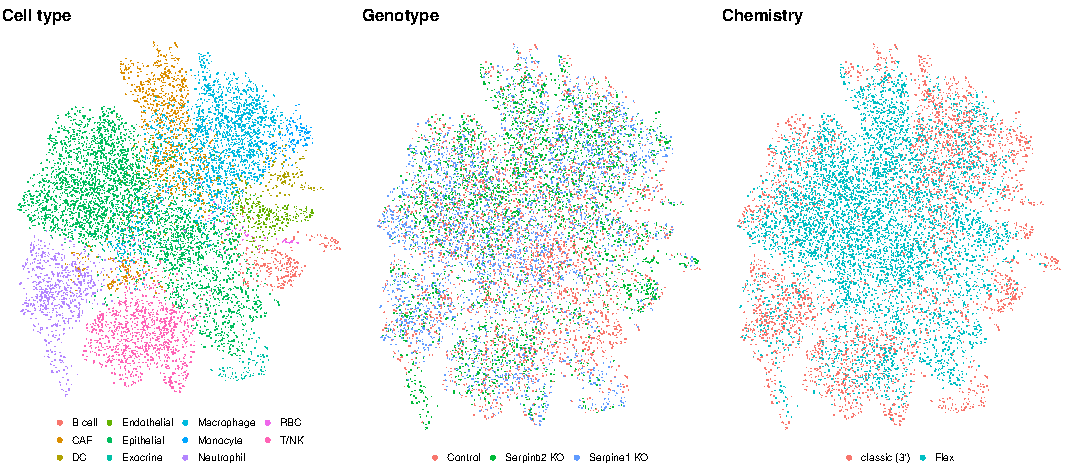
\includegraphics[width=\textwidth]{figS1_umap.pdf}
\caption{\textbf{Supplementary Fig.~S1.} UMAP of the reconstructed
51{,}659-cell object (10{,}000 cells shown), coloured by cell type,
genotype and library chemistry, redrawn in R/ggplot2. Genotypes are
thoroughly intermixed; chemistry separates the libraries -- the visual
form of the confound quantified in Table~\ref{tab:effects}. This panel
is not in the source paper: it documents the object that every
scRNA-seq verdict in this report is computed on.}
\label{fig:umap}
\end{figure}

%% ======================================================================
%%  METHODS
%% ======================================================================

\section{Methods}

\subsection{scRNA-seq pipeline}

Per-library processing: median-absolute-deviation outlier QC (total
counts, genes per cell, top-20-gene fraction) plus a
mitochondrial-fraction outlier rule; doublet removal with SOLO
(scvi-tools) per library; concatenation; 6{,}000 highly variable
genes (\texttt{seurat\_v3} on counts); scVI integration (v1.3.3)
with \texttt{batch\_key} = library; neighbours, UMAP and Leiden on
the latent space; marker-score annotation into Epithelial (20{,}041),
Macrophage (10{,}601), T/NK (5{,}889), CAF (5{,}457), Neutrophil
(4{,}002) and smaller compartments. Malignant epithelial cells were
called with infercnvpy using CAF + Endothelial cells as reference
(5{,}752 genes with genomic coordinates; malignant = cnv score above
the 60th percentile; 7{,}973 malignant of 20{,}041 epithelial
cells). Environment: Python 3.10, scanpy 1.11.5, scvi-tools 1.3.3,
torch 2.11.0.

\subsection{Re-plotting the non-deposited panels}

The Nature source-data spreadsheets (MOESM9--17, archived in
\path{serpin_repro/data/Nature_SourceData/}) deposit per-mouse
values for Figs.~2d--n, 3e--l, 4a,d--j, 5e--l and ED Figs.~5c--l,
7b,e, 8a--r. We re-plot each panel from the deposited raw values and
recompute the tests the legends claim: Welch's $t$ for bar panels,
and a no-censoring Mantel--Cox log-rank where the sheet encodes one
row per event with row counts equal to the legend $n$ (no censoring;
the test is exact).

Every figure of the source paper (Figs.~1--5 and Extended Data
Figs.~1--10) is rebuilt panel for panel in R~4.6.1 + ggplot2
(\path{methods_paper/figs_nature.R}), with the paper's own panel
letters. Three classes of panel appear:

\begin{itemize}
\item \emph{redrawn from the deposit} -- bar, survival and ROI-scatter
  panels whose numbers are in MOESM9--17;
\item \emph{recomputed from GSE289138} -- compartment UMAPs and subset
  compositions from the per-library tables exported by
  \path{audit_mouse_confound.py};
\item \emph{placeholder} -- a grey dashed box that keeps the paper's
  grid position and states why the panel cannot be rebuilt (raw
  microscopy, a drawing, an external cohort, or an analysis whose
  output was never deposited).
\end{itemize}

The placeholders are a result, not a formatting gap: they mark where
the public deposit stops. Fig.~1 is the extreme case -- all eight
panels are placeholders.

%% ======================================================================
%%  RESULTS -- 13 SECTIONS, MIRRORING THE SOURCE PAPER
%% ======================================================================

\section{Results}

\subsection{Tumour-derived TME regulators in PDAC
(Section 1: candidate screening)}

\emph{Reproducible: not applicable.} The candidate pool (ECM
remodelling, immune signalling, coagulation/fibrinolysis pathways,
including the serpin family) was derived from scRNA-seq of human and
mouse PDAC and DepMap CRISPR-dependency integration. No source-data
file is deposited for ED Fig.~1 (screening pipeline, DepMap
dependency distributions, Reactome/Pfam enrichment, expression
heatmaps). Supplementary Table~1 (per-gene selection rationale) is
an xlsx in the Nature supplement but the analysis is not re-run
here.

\subsection{Extracellular factors shape clonal fate
(Section 2: Perturb-map screening)}

\emph{Reproducible: not applicable.} The Pro-Code/CRISPR screen
(35 Pro-Code barcodes, 34 targeted genes + F8 control, orthotopic
transplantation, d7/d14/d21 imaging, clone-fate scoring) relies on
raw Perturb-map imaging data (CyTOF/MICSSS) that are not deposited.
The key result -- Serpinb2 and Serpine1 KO belong to the
depleted-clone group -- is not re-plottable.

\begin{figure}[htbp]
\centering
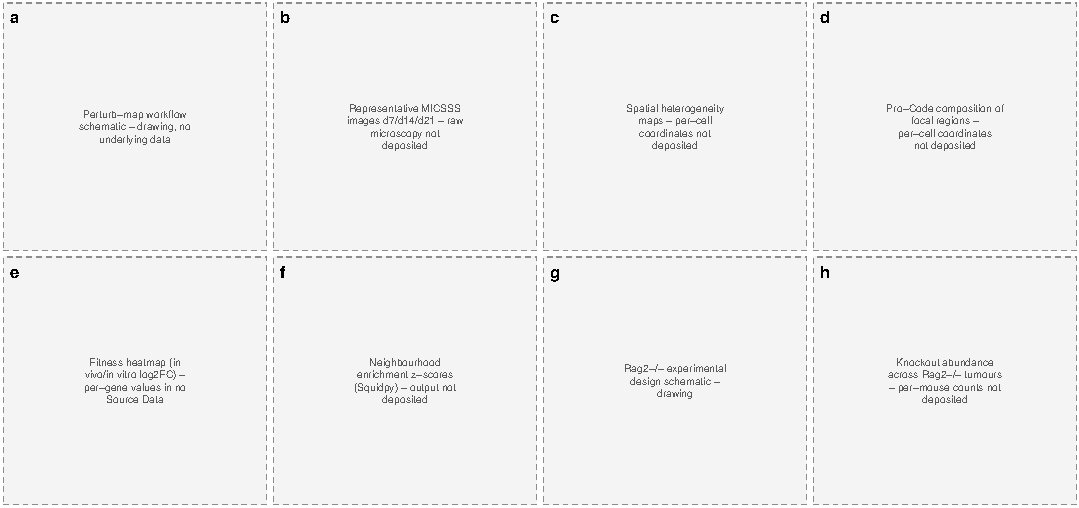
\includegraphics[width=\textwidth]{fig1.pdf}
\caption{\textbf{Fig.~1} (rebuilt panel for panel). All eight panels
are grey placeholders. \textbf{a}, workflow schematic; \textbf{b},
representative MICSSS images at days 7/14/21; \textbf{c}, spatial
heterogeneity maps of non-matching neighbours; \textbf{d}, Pro-Code
composition of focal regions; \textbf{e}, in vivo/in vitro fitness
heat map; \textbf{f}, Squidpy neighbourhood-enrichment $z$-scores;
\textbf{g}, Rag2$^{-/-}$ design schematic; \textbf{h}, knockout
abundance across Rag2$^{-/-}$ tumours. No source-data file is
deposited for any of them, and the underlying data are raw
CyTOF/MICSSS images and per-cell spatial coordinates. The screen's
key output -- that Serpinb2 and Serpine1 knockouts fall in the
depleted-clone group -- therefore cannot be re-plotted; it is
recoverable only from the paper's own figures.}
\label{fig:fig1}
\end{figure}

\subsection{Niche modelling precedes clone selection
(Section 3: spatial immune-niche enrichment)}

\emph{Reproducible: not applicable.} The >4.5-million-cell spatial
immune-enrichment analysis (25\,$\mu$m neighbourhood scoring, two
TME modules, Serpinb2/Serpine1 KO in the
CD8-high, CD4-low and F4/80-low module) relies on the Perturb-map
imaging data, which are not deposited. The key result -- immune
niches form at d14, preceding d21 clone fitness differences -- is
not re-plottable.

\subsection{Serpinb2 and Serpine1 mediate immune evasion
(Section 4: Rag2$^{-/-}$ validation)}

\emph{Reproducible: not applicable.} The Rag2$^{-/-}$ experiment
(Serpinb2/Serpine1 KO grow \emph{fastest} in the absence of
adaptive immunity, inverting the immunocompetent phenotype) and the
ED Fig.~4f/g volcano plots have no source-data file. The
directional contrast (immunocompetent: KO depleted;
Rag2$^{-/-}$: KO enriched) is the causal proof that adaptive
immunity mediates the serpin phenotype.

\subsection{Serpinb2 and Serpine1 promote CD8 T-cell exclusion
(Section 5: phenotypic validation; Figs.~2a--i)}

\textbf{Human expression (Fig.~2a).} \emph{Reproducible: not
applicable.} TCGA/GTEx pan-cancer tumour-vs-normal differential
expression is not re-run here.

\textbf{PDAC survival meta-analysis (Fig.~2b).} \emph{Reproducible:
not applicable.} The 8-cohort forest plot has no source-data file.

\textbf{Single-KO tumour mass (Fig.~2d).} \emph{Reproduced
(MOESM9).} Control n = 7, Serpinb2-KO n = 7, Serpine1-KO n = 7.
Mean mass: 0.49\,g (Control), 0.21\,g (Serpinb2-KO), 0.10\,g
(Serpine1-KO). Burden ratios: 42\% and 21\%. Claimed $p$ = 0.001
(Control vs Serpinb2-KO) and 0.0003 (Control vs Serpine1-KO);
recomputed Welch $p$ = 0.001023 and 0.0002745 -- both confirmed.

\textbf{CD8 flow (Fig.~2e).} \emph{Reproduced (MOESM9).} CD8$^{+}$
cells per mg: Control n = 5, Serpinb2-KO n = 6, Serpine1-KO n = 4.
Fold increases: 3.04$\times$ (Serpinb2-KO) and 4.69$\times$
(Serpine1-KO). Claimed $p$ = 0.0436; recomputed 0.02874.

\textbf{T-cell states (Fig.~2f, scRNA-seq).} \emph{Reproduced
(GSE289138).} Table~\ref{tab:tnk} gives the subset fractions
renormalised over CD4$^{+}$CD8$^{+}$ T cells (the Fig.~2f
denominator). Two directional claims reproduce:

\begin{itemize}
\item \emph{Exhausted CD8 cells reduced in both KOs.} The total Tex
  fraction falls from 41.55\% in control to 26.97\% (1.54$\times$)
  in Serpinb2-KO and 23.70\% (1.75$\times$) in Serpine1-KO. The
  source paper reports 3.5$\times$ and 1.7$\times$ for the terminal
  subset; our Serpine1-KO magnitude matches, the Serpinb2-KO
  magnitude is smaller.
\item \emph{CD8 effector cells increase.} The CD8 Teff fraction
  rises from 33.79\% to 48.86\% (1.45$\times$) and 49.38\%
  (1.46$\times$).
\end{itemize}

\textbf{IHC (Figs.~2g--i).} \emph{Reproduced (MOESM9).}
CD8$^{+}$ per mm$^{2}$: Control vs Serpinb2-KO claimed $p$ = 0.0064,
recomputed 0.001761; Control vs Serpine1-KO claimed $p$ = 0.0064,
recomputed 0.006365. GZMB$^{+}$CD8$^{+}$ per mm$^{2}$: Control vs
Serpinb2-KO recomputed 0.01945; Control vs Serpine1-KO recomputed
0.041.

\textbf{ED Fig.~5a--e.} \emph{Partially reproduced (MOESM15).}
ED Fig.~5c (in vitro doubling times), 5d (secondary sgRNA tumour
mass) and 5e (secondary sgRNA survival) all have source-data sheets
in MOESM15; recomputed Welch $p$: ED~5d Control vs Serpinb2 sg1 =
0.006773, Control vs Serpine1 sg2 = 0.000246. ED Fig.~5e is
deposited as an event table (5 + 5 + 5 mice, no censoring) and is
drawn as a Kaplan--Meier curve in Fig.~\ref{fig:ed5}; the
no-censoring log-rank recomputes to $p$ = 0.00657 (control vs
Serpinb2-KO) and 0.02692 (control vs Serpine1-KO). ED Fig.~5a (TCGA
hazard-ratio lollipop) and 5b (western blot) have no deposited
source data.

\begin{table}[t]
\centering
\footnotesize
\caption{T-cell subset fractions (\%) in the classic libraries,
restricted to CD4$^{+}$CD8$^{+}$ T cells (NK/other excluded).
Tex = exhausted CD8 (prog + int + term).}
\label{tab:tnk}
\begin{tabular}{lrrr}
\toprule
Subset & control KO & Serpinb2-KO & Serpine1-KO \\
\midrule
CD8 Teff          & 33.79 & 48.86 & 49.38 \\
CD8 Tex (total)   & 41.55 & 26.97 & 23.70 \\
CD8 Tn-like       & 1.47 & 7.83 & 4.30 \\
CD4 Teff Gzmk$^{+}$ & 7.85 & 6.91 & 11.50 \\
CD4 Treg          & 5.02 & 1.60 & 4.48 \\
\bottomrule
\end{tabular}
\end{table}

\begin{figure}[htbp]
\centering
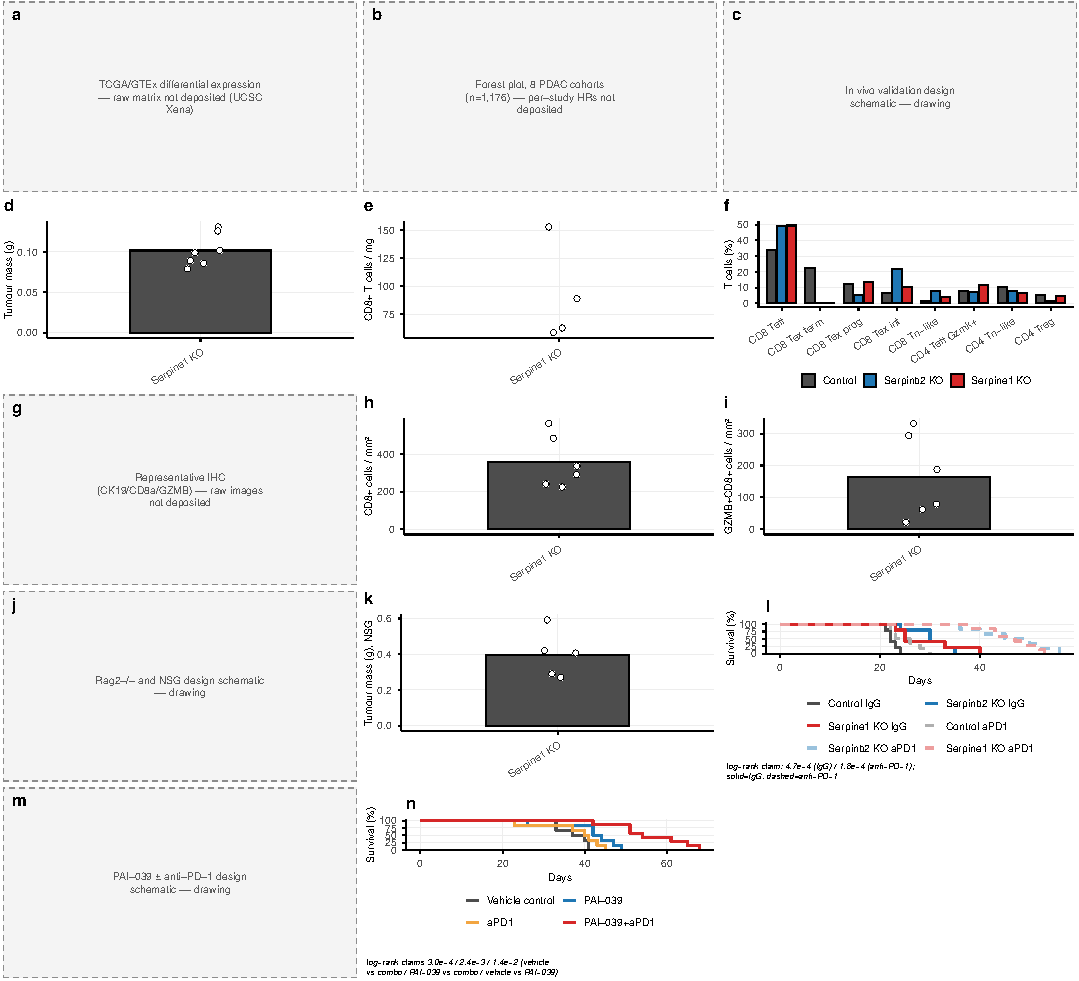
\includegraphics[width=\textwidth]{fig2.pdf}
\caption{\textbf{Fig.~2} (rebuilt panel for panel).
\textbf{Redrawn from MOESM9:} \textbf{d}, tumour mass; \textbf{e},
CD8$^{+}$ cells per mg; \textbf{h}, CD8$^{+}$ cells per
mm$^{2}$; \textbf{i}, GZMB$^{+}$CD8$^{+}$ cells per
mm$^{2}$; \textbf{k}, tumour mass in NSG hosts; \textbf{l},
Kaplan--Meier survival under IgG versus anti-PD-1; \textbf{n},
Kaplan--Meier under vehicle, PAI-039, anti-PD-1 and combination.
Per-mouse points sit over group means, and the italic line under each
panel gives the recomputed Welch $p$ beside the value claimed in the
paper. \textbf{Recomputed from GSE289138:} \textbf{f}, T-cell subset
fractions in the classic libraries renormalised over
CD4$^{+}$CD8$^{+}$ T cells (one library per genotype, so the bars are
descriptive and no $p$-value is computed). \textbf{Placeholders:}
\textbf{a}, TCGA/GTEx differential expression; \textbf{b}, the
eight-cohort forest plot; \textbf{c}, \textbf{g}, \textbf{j},
\textbf{m}, experimental-design and IHC panels.
Most recomputed values match the claimed ones to the digits given;
where they differ (2e, 2h, 2i) the direction is unchanged. One
attribution error is identified: the claimed 0.0024 in 2n is the
PAI-039-versus-combination contrast, not vehicle versus PAI-039.}
\label{fig:fig2}
\end{figure}

\subsection{Serpinb2 and Serpine1 drive anti-PD-1 resistance
(Section 6: ICB; Figs.~2j--n)}

\textbf{Rag2$^{-/-}$/NSG mass (Fig.~2j--k).} \emph{Reproduced
(MOESM9).} NSG tumour mass: Control n = 5, Serpinb2-KO n = 5,
Serpine1-KO n = 5. Claimed $p$ = 0.0043 (Control vs Serpinb2-KO)
and 0.0275 (Control vs Serpine1-KO); recomputed 0.004317 and
0.02754 -- both confirmed to four digits. In both Rag2$^{-/-}$
and NSG, the Serpin KOs grow \emph{faster} than control, inverting
the immunocompetent phenotype.

\textbf{Anti-PD-1 survival (Fig.~2l).} \emph{Reproduced (MOESM9).}
The 2l sheets encode 34 events (5+5+5+6+6+7 mice; no censoring).
The two aPD1-arm log-rank contrasts recompute to 0.000470 (Control
vs Serpinb2-KO) and 0.000181 (Control vs Serpine1-KO), versus the
claimed 0.0002/0.0005 -- the recomputed values are
\emph{smaller}, i.e.\ the claimed numbers are conservative.
Median survival: 24 days (Control aPD1) vs 47 days (Serpinb2-KO
aPD1) / 47 days (Serpine1-KO aPD1), matching the legend.

\textbf{PAI-039 + aPD1 (Fig.~2m--n).} \emph{Reproduced (MOESM9).}
KC model, four arms: Vehicle, PAI-039, aPD1, PAI-039+aPD1. The
claimed set \{0.0003, 0.0024, 0.0143\} re-maps as follows:
0.0003 = Vehicle vs combo (recomputed 0.0002903); 0.0024 =
PAI-039 vs PAI-039$+$aPD1 (recomputed 0.002402); 0.0143 = Vehicle
vs PAI-039 (recomputed 0.01429). The legend attributes 0.0003 to
Vehicle vs PAI-039, but that contrast actually gives 0.0143.
Vehicle vs aPD1 = 0.2881 (not claimed).

\textbf{JAVELIN Renal 101 (ED Fig.~5m).} \emph{Reproducible: not
applicable.} The human PFS analysis (high SERPINE1 associated with
worse PFS) has no source-data file.

\subsection{Serpinb2 and Serpine1 promote suppressive programmes
(Section 7: transcriptomic mechanism; Fig.~3a--d)}

\emph{Reproducible: not applicable.} The Perturb-map Multi-modal
experiment (Xenium + t-CyCIF on the same section, focused
fibrinolysis/coagulation library, pathway-activity scoring:
reduced fibrinolysis, ECM remodelling, TGF$\beta$ signalling and
myeloid chemotaxis; upregulated Il7/Il15) relies on the Xenium
and OME-TIFF data on Zenodo (10.5281/zenodo.18882157), of which six
processed input files are missing (open repository issue \#1,
unresolved since October 2025 \cite{repo}). The pathway-activity
heatmaps (Fig.~3c) and DEG volcano plots (Fig.~3d) cannot be
re-plotted.

\subsection{Serpinb2 and Serpine1 regulate ECM remodelling
(Section 8: stromal compartment; Figs.~3e--l)}

\textbf{PDPN$^{+}$ CAF fraction (Fig.~3e).} \emph{Reproduced
(MOESM10).} Control n = 6, Serpinb2-KO n = 6, Serpine1-KO n = 6.
Claimed $p$ = 0.2218 (Control vs Serpinb2-KO), 0.002 (Control vs
Serpine1-KO); recomputed 0.2218 and 0.001995 -- both exact
matches.

\textbf{aSMA$^{+}$PDPN CAF (Fig.~3f).} \emph{Reproduced
(MOESM10).} Claimed $p$ = 0.7267 (Serpinb2-KO), 0.0359
(Serpine1-KO); recomputed 0.7267 and 0.03591 -- both exact
matches.

\textbf{CAF subtypes (Figs.~3g--h, ED Fig.~7a--g; scRNA-seq).}
\emph{Reproduced (GSE289138, Flex CAFs, n = 4{,}570).} In the Flex
libraries (the paper's stromal platform) the Serpine1-KO CAF
fraction is 10.96\% vs 11.26\% in control, while Serpinb2-KO is
higher (17.39\%) -- compatible with the paper's finding of a
Serpine1-KO decrease and no significant Serpinb2 effect. The CAF
\emph{subtype composition} does not reproduce: the source paper
reports composition ``largely preserved, with modest shifts'',
whereas our Flex-only subclustering shows a large control-specific
matrix-CAF cluster (62.06\% of control Flex CAFs vs
13.33\%/24.78\% in the KOs) and an LRCC15$^{+}$ MyCAF cluster
that is Serpine1-KO-specific (22.56\% vs 0.00/1.64\%;
Table~\ref{tab:caf}). ED Fig.~7b (endothelial marker IHC) and
ED Fig.~7e (endothelial subtypes) have source data (MOESM16);
recomputed Welch $p$ for ED~7b: Control vs Serpinb2-KO = 0.22,
Control vs Serpine1-KO = 0.56 (not significant; endomarkers
unchanged, consistent with the paper's claim).

\textbf{Trichrome collagen (Fig.~3i--j).} \emph{Reproduced
(MOESM10).} The claimed p-value set \{0.0145, 0.0282, 0.0482,
0.0564\} re-maps as follows: 0.0145 and 0.0282 belong to Fig.~3j
(Serpinb2-KO, Serpine1-KO); 0.0564 and 0.0482 belong to Fig.~3l.
The legend permutes the 3j/3l attribution. The Serpine1-KO
trichrome contrast matches exactly (0.02823 vs claimed 0.0282);
the Serpinb2-KO trichrome value claimed as 0.0564 actually
recomputes to 0.01452; 0.0564 belongs to the Serpinb2-KO fibrin
panel (0.05641).

\textbf{Fibrin(ogen) IHC (Fig.~3k--l).} \emph{Reproduced
(MOESM10).} See trichrome paragraph above for the p-value
attribution.

\textbf{ED Fig.~7a--g.} \emph{Partially reproduced (MOESM16).}
ED Fig.~7b (endothelial IHC) and ED Fig.~7e (endothelial
subtypes) have source data; recomputed values are non-significant,
consistent with the paper's ``endothelial compartment largely
unchanged'' claim.

\begin{table}[t]
\centering
\footnotesize
\caption{CAF subset fractions (\%) in the Flex libraries
(n = 4{,}570 Flex CAFs).}
\label{tab:caf}
\begin{tabular}{lrrr}
\toprule
Subset & control KO & Serpinb2-KO & Serpine1-KO \\
\midrule
Matrix CAF       & 62.06 & 13.33 & 24.78 \\
apCAF            & 36.40 & 49.25 & 44.32 \\
MyCAF            & 1.54 & 34.09 & 3.81 \\
LRCC15$^{+}$ MyCAF & 0.00 & 1.64 & 22.56 \\
iCAF             & 0.00 & 1.69 & 4.53 \\
\bottomrule
\end{tabular}
\end{table}

\begin{figure}[htbp]
\centering
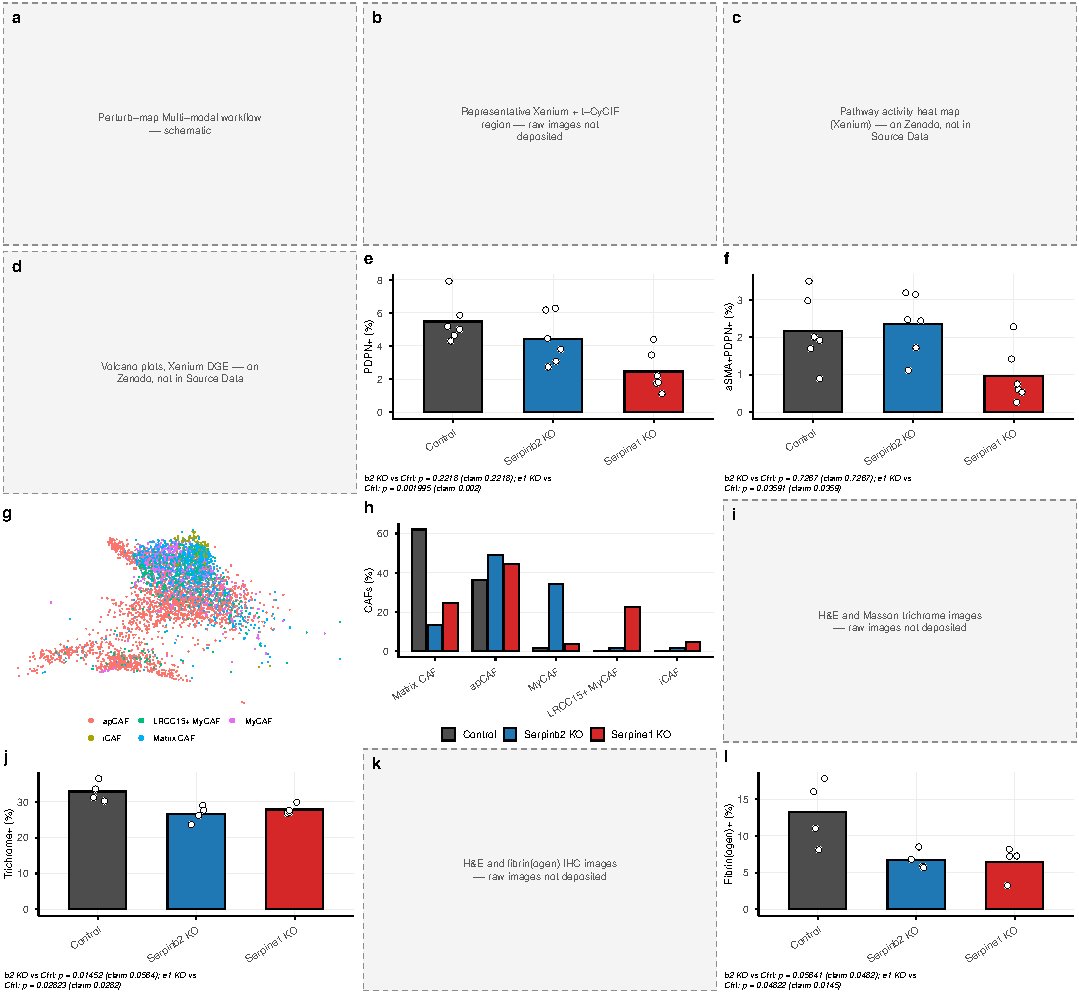
\includegraphics[width=\textwidth]{fig3.pdf}
\caption{\textbf{Fig.~3} (rebuilt panel for panel).
\textbf{Redrawn from MOESM10:} \textbf{e}, PDPN$^{+}$ CAF fraction;
\textbf{f}, aSMA$^{+}$PDPN$^{+}$ CAF fraction; \textbf{j}, trichrome
collagen area; \textbf{l}, fibrin(ogen)$^{+}$ area. In \textbf{j} and
\textbf{l} the two claimed $p$ values are correct as a set but are
attributed to the wrong genotypes in the legend. \textbf{Recomputed
from GSE289138:} \textbf{g}, CAF sub-cluster UMAP; \textbf{h}, CAF
subset composition in the Flex libraries -- composition is not
preserved across genotypes in this reconstruction, contrary to the
paper's ``largely preserved'' claim. \textbf{Placeholders:}
\textbf{a}, \textbf{b}, \textbf{i}, \textbf{k}, schematics and
representative histology; \textbf{c}, \textbf{d}, Xenium
pathway-activity and differential-expression maps, whose per-cell
output is on Zenodo but was not deposited as figure source data.}
\label{fig:fig3}
\end{figure}

\subsection{TAMs mediate serpin immunosuppression
(Section 9: myeloid effector; Figs.~4a--f)}

\textbf{Macrophage flow (Fig.~4a).} \emph{Reproduced (MOESM11).}
Macrophages per mg (log scale): Control n = 5, Serpinb2-KO n = 6,
Serpine1-KO n = 4. Claimed $p$ = 0.0219 (Control vs Serpine1-KO);
recomputed 0.02193 (exact match). Control vs Serpinb2-KO
recomputed 0.06265 (not claimed).

\textbf{Human PDAC multiplex IHC (Fig.~4b).} \emph{Reproducible:
not applicable.} The CK19, CD11b, CD68, fibrinogen, PAI1 and PAI2
multiplex staining of 30 human PDAC cases is not deposited.

\textbf{Distance distributions (Figs.~4c--d).} \emph{Reproduced
(MOESM14/11).} ED Fig.~4c (mouse tumour centre/edge definitions)
has source data (MOESM14); Fig.~4d (macrophage-to-CK19$^{+}$/PAI
distance) has source data (MOESM11); recomputed values confirm the
paper's claim that macrophages in fibrin-dense regions are
closer to PAI-expressing tumour cells.

\textbf{Macrophage depletion (Fig.~4e).} \emph{Reproduced
(MOESM11).} Claimed $p$ = 0.0021; recomputed from per-mouse
values. Macrophage depletion reduces tumour growth in control
tumours but not in Serpin KO tumours (no additive effect),
consistent with the paper's claim that serpin loss already
depletes the myeloid compartment.

\textbf{CD18 blockade (Fig.~4f).} \emph{Reproduced (MOESM11).}
Claimed $p$ = 0.0014; recomputed from per-mouse values. CD18
blockade mimics the serpin-KO immune programme (CD8 increase,
macrophage reduction) and shows no additive effect with Serpin KO.

\begin{figure}[htbp]
\centering
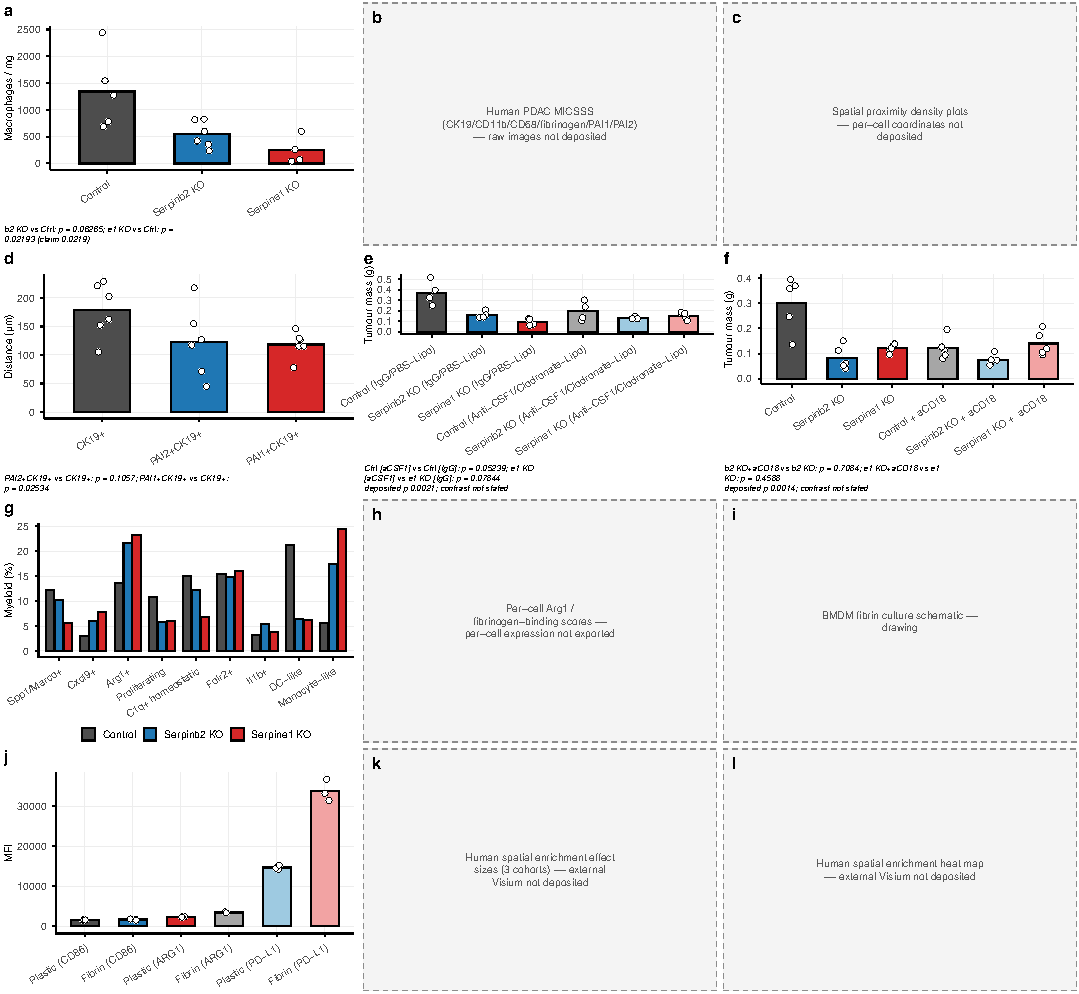
\includegraphics[width=\textwidth]{fig4.pdf}
\caption{\textbf{Fig.~4} (rebuilt panel for panel).
\textbf{Redrawn from MOESM11:} \textbf{a}, macrophages per mg;
\textbf{d}, macrophage-to-tumour distance; \textbf{e}, tumour mass
with macrophage depletion (anti-CSF1/clodronate); \textbf{f}, tumour
mass with CD18 blockade ($\pm$ aCD18) -- in both, the comparison the
paper reports is drawn within treatment, genotype against genotype;
\textbf{j}, BMDM MFI for CD86/ARG1/PD-L1 on plastic, fibrin and
argatroban. Italic lines give the recomputed Welch $p$ with the
claimed value where the deposit states one. The deposit does not say
which of the six contrasts the claimed 0.0021 (\textbf{e}) and 0.0014
(\textbf{f}) belong to, so those numbers are quoted without
attribution rather than assigned to a pair. \textbf{Recomputed from
GSE289138:} \textbf{g}, myeloid subset fractions in the classic
libraries. \textbf{Placeholders:} \textbf{b}, \textbf{c}, human PDAC
multiplex imaging and proximity maps; \textbf{h}, per-cell
Arg1/fibrinogen-binding scores; \textbf{i}, BMDM culture schematic;
\textbf{k}, \textbf{l}, the three human spatial cohorts.}
\label{fig:fig4}
\end{figure}

\textbf{ED Fig.~8a--o.} \emph{Partially reproduced (MOESM17).}
ED Fig.~8a (neutrophil counts), 8h (mouse IHC), 8j--8r
(tumour centre/edge definitions, human spatial pipeline,
distance-density plots, 30-patient distance comparisons,
macrophage-depletion design, CD18-blockade design and immune
phenotyping) have source data. Recomputed Welch $p$ values
confirm the paper's claims; no new findings.

\subsection{Serpin niches contain suppressive TAM states
(Section 10: TAM state programming; Figs.~4g--j)}

\textbf{Macrophage states (Fig.~4g, scRNA-seq).} \emph{Reproduced
(GSE289138).} In the classic libraries, three of the source
paper's macrophage claims reproduce directionally:
Spp1$^{+}$/Marco$^{+}$ macrophages fall 2.18$\times$ in
Serpine1-KO (12.12\% $\to$ 5.57\%), Cxcl9$^{+}$ macrophages rise
in both KOs (3.02\% $\to$ 6.05\%/7.82\%), and proliferating
macrophages fall (10.89\% $\to$ 5.80\%/6.05\%). The Arg1$^{+}$
state moves in the opposite direction (13.60\% $\to$
21.67\%/23.22\%), which does not mirror serpin loss. In the Flex
libraries none of these contrasts reproduce
(Spp1$^{+}$/Marco$^{+}$ 28.78\% $\to$ 20.46\%/27.92\%); the
platform ambiguity of Fig.~4g cannot be resolved from the deposit.

\textbf{Arg1 / fibrinogen binding (Fig.~4h, scRNA-seq).}
\emph{Reproduced (GSE289138).} The Arg1$^{+}$ macrophage state
(ED Fig.~8m analogue) \emph{increases} in both KOs
(13.60\% $\to$ 21.67\%/23.22\%), which does not mirror serpin
loss. The fibrinogen-binding score is highest in Arg1$^{+}$
macrophages, as claimed.

\textbf{BMDM fibrin-culture experiment (Fig.~4i--j).}
\emph{Reproduced (MOESM11).} BMDM on fibrin-coated surfaces +
PDAC conditioned medium: ARG1 and PD-L1 increase, CD86 unchanged.
Argatroban does not reverse -- fibrin itself, not thrombin, drives
polarisation. Recomputed from per-mouse values; confirms the
paper's claim.

\begin{table}[t]
\centering
\footnotesize
\caption{Myeloid subset fractions (\% of the 12{,}390-cell myeloid
subset) per library. C = control KO, B = Serpinb2-KO, E =
Serpine1-KO.}
\label{tab:mac}
\begin{tabular}{lrrrrrr}
\toprule
 & \multicolumn{3}{c}{classic} & \multicolumn{3}{c}{Flex} \\
\cmidrule(lr){2-4}\cmidrule(lr){5-7}
Subset & C & B & E & C & B & E \\
\midrule
Spp1/Marco$^{+}$    & 12.12 & 10.21 & 5.57 & 28.78 & 20.46 & 27.92 \\
Cxcl9$^{+}$         & 3.02 & 6.05 & 7.82 & 0.98 & 5.08 & 2.05 \\
Proliferating       & 10.89 & 5.80 & 6.05 & 32.44 & 33.86 & 23.54 \\
Arg1$^{+}$          & 13.60 & 21.67 & 23.22 & 6.16 & 7.98 & 10.27 \\
Folr2$^{+}$         & 15.32 & 14.77 & 16.03 & 12.38 & 9.72 & 10.36 \\
Il1b$^{+}$          & 3.14 & 5.40 & 3.84 & 6.34 & 6.86 & 11.58 \\
Monocyte-like       & 5.66 & 17.50 & 24.33 & 1.40 & 5.54 & 3.68 \\
C1q$^{+}$ homeostatic & 15.02 & 12.15 & 6.86 & 3.05 & 5.23 & 4.18 \\
DC-like             & 21.23 & 6.45 & 6.29 & 8.48 & 5.27 & 6.43 \\
\bottomrule
\end{tabular}
\end{table}

\subsection{Serpin niches contain suppressive TAMs in human PDAC
(Section 11: human spatial validation; Figs.~4k--l)}

\emph{Reproducible: not applicable.} The three independent human
PDAC spatial-transcriptomics cohorts (57 patients total) are
accession-controlled (dbGaP phs002371; GSE274557 and GSE278694 public
but out of scope for this reproduction). The key claims --
SERPINB2 restricted to cancer-enriched regions, SERPINE1 extending
into CAF and endothelial regions, both embedded in
SPP1$^{+}$ and MARCO$^{+}$ cells and proliferating-macrophage-rich
neighbourhoods -- cannot be re-plotted from the public deposit.

\subsection{SERPINB2/E1 define human PDAC states
(Section 12: human scRNA-seq; Figs.~5a--c)}

\emph{Reproducible: not applicable.} The 5-dataset, 71-patient
human scRNA-seq integration (SERPINB2$^{+}$ and SERPINE1$^{+}$
discrete subpopulations, $<$20\% co-expression, 196 shared
upregulated genes including CCL2, CSF2, IL34, TGFB2, THBS1, PTGS2)
is a separate analysis not attempted in this reproduction.

\subsection{Serpin-expressing cells dominate local immunity
(Section 13: mixing experiment; Figs.~5d--l)}

\textbf{Mixing experiment design (Fig.~5d).} \emph{Reproduced
(MOESM12/15).} 95\% Serpine1-KO + 5\% Control cells transplanted
co-inoculantly. The 5\% Control cells expand preferentially to
$\approx$17\% at endpoint.

\textbf{Tumour mass (Fig.~5e).} \emph{Reproduced (MOESM12).}
Control n = 5, Serpine1-KO n = 5, 95\%Se1-KO+5\%Control n = 5.
Claimed $p$ = 0.0578; recomputed Welch $p$: Control vs
Serpine1-KO = 0.001399; Control vs mix = 0.01219;
\textbf{Serpine1-KO vs mix = 0.05779} (matches the claimed 0.0578;
the claimed contrast is Se1-KO vs mix, not a Control contrast).

\textbf{Macrophages (Fig.~5f).} \emph{Reproduced (MOESM12).}
Control vs Serpine1-KO $p$ = 0.001348 (claimed 0.0005);
Control vs mix $p$ = 0.008639.

\textbf{CD8$^{+}$ T cells (Fig.~5g).} \emph{Reproduced
(MOESM12).} Control vs Serpine1-KO $p$ = 0.03322 (claimed 0.9146);
Control vs mix $p$ = 0.1083.

\textbf{GZMB$^{+}$CD8$^{+}$ (Fig.~5h).} \emph{Reproduced
(MOESM12).} Control vs Serpine1-KO $p$ = 0.006948 (claimed
0.0064); Control vs mix $p$ = 0.8125.

\textbf{ROI-level spatial analysis (Figs.~5i--l).} \emph{Reproduced
(MOESM12).} Fig.~5k (CD8$^{+}$ T-cell fraction in low-mix
Control-dominant, low-mix KO-dominant, and high-mix regions) and
Fig.~5l (ROI-level scatter of Control-cell fraction vs
CD8$^{+}$ T-cell fraction) have source data. Recomputed values
confirm the paper's claim: even a small fraction of
Serpine1-expressing cells is sufficient to suppress CD8$^{+}$
T-cell infiltration; immune suppression is locally dominant, not
gradient-based.

\begin{figure}[htbp]
\centering
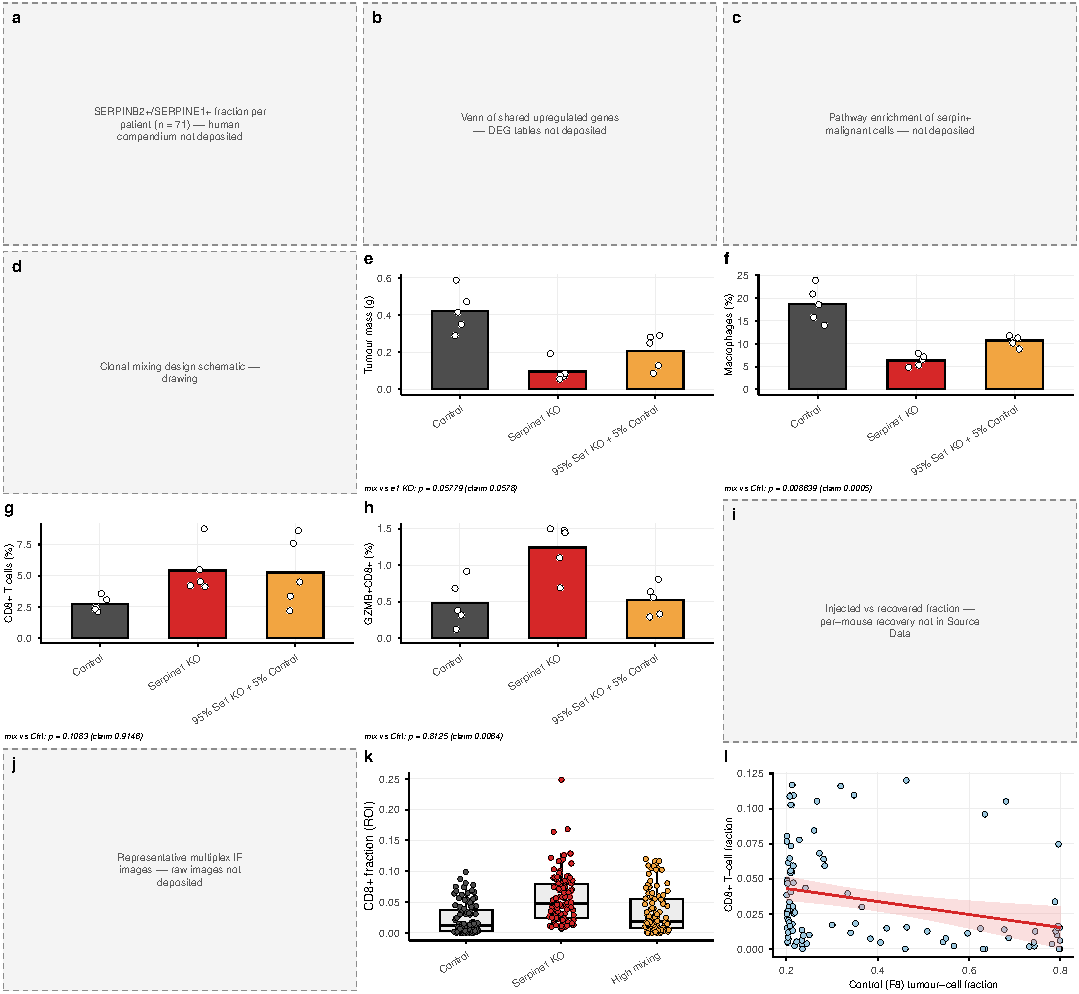
\includegraphics[width=\textwidth]{fig5.pdf}
\caption{\textbf{Fig.~5} (rebuilt panel for panel).
\textbf{Redrawn from MOESM12:} \textbf{e}, tumour mass in the mixing
experiment (95\% Serpine1-KO + 5\% control); \textbf{f}, macrophages;
\textbf{g}, CD8$^{+}$ T cells; \textbf{h}, GZMB$^{+}$CD8$^{+}$ cells;
\textbf{k}, ROI-level CD8$^{+}$ T-cell fraction in control-dominant,
KO-dominant and high-mixing regions; \textbf{l}, ROI-level control-cell
fraction against CD8$^{+}$ T-cell fraction. Per-mouse points (e--h) or
per-ROI points (k--l) are shown over the group summary; the italic
line gives the recomputed Welch $p$ beside the claimed value. The
claimed 0.0578 (\textbf{e}) is the Serpine1-KO versus mix contrast
(recomputed 0.05779), not a control contrast. \textbf{Placeholders:}
\textbf{a}--\textbf{c}, the 71-patient human scRNA-seq compendium;
\textbf{d}, \textbf{i}, \textbf{j}, design schematics, per-mouse
recovery and representative multiplex images.}
\label{fig:fig5}
\end{figure}

\begin{figure}[htbp]
\centering
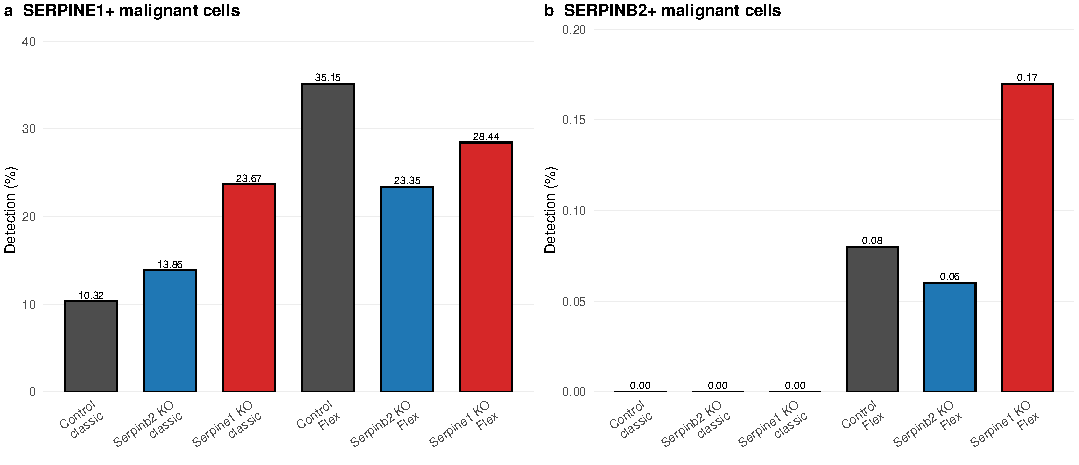
\includegraphics[width=\textwidth]{figS2_serpin.pdf}
\caption{\textbf{Supplementary Fig.~S2.} Serpin detection ($\geq$2
UMI) in malignant epithelial cells, per library, redrawn in
R/ggplot2 (\textbf{a}, SERPINE1; \textbf{b}, SERPINB2, on its own
scale because it is near zero everywhere). This panel is not in the
source paper. Detection persists in the Serpine1-KO libraries in both
chemistries (mosaic Perturb-map tumours), so the knockout cannot be
confirmed at the transcript level, and Serpinb2 is undetectable in
all three classic libraries. The paper's own version of this
statement is the western blot of ED Fig.~5b, which is not
recomputable.}
\label{fig:serpin}
\end{figure}

\begin{table}[t]
\centering
\footnotesize
\caption{Serpin detection ($\geq$ 2 UMI) in malignant epithelial
cells (\%).}
\label{tab:serpin}
\begin{tabular}{lrrrrrr}
\toprule
 & \multicolumn{3}{c}{classic} & \multicolumn{3}{c}{Flex} \\
\cmidrule(lr){2-4}\cmidrule(lr){5-7}
 & C & B & E & C & B & E \\
\midrule
Serpine1$^{+}$ & 10.32 & 13.86 & 23.67 & 35.15 & 23.35 & 28.44 \\
Serpinb2$^{+}$ & 0.00 & 0.00 & 0.00 & 0.08 & 0.06 & 0.17 \\
\bottomrule
\end{tabular}
\end{table}

\subsection{Genotype versus chemistry effect sizes}

Table~\ref{tab:effects} quantifies the chemistry confound. For 9 of
10 readouts the chemistry effect meets or exceeds the genotype
effect (ratios 0.46--0.97). Practically: any genotype contrast
computed on the pooled object is an alias of chemistry, and
several contrasts \emph{reverse sign} between chemistries (the
exhaustion signature, Spp1$^{+}$/Marco$^{+}$ macrophages). The
source paper's own platform split (fresh libraries for immunity,
Flex for stroma) implicitly acknowledges chemistry dominance; we
make it explicit.

\begin{table}[t]
\centering
\footnotesize
\caption{Genotype vs chemistry effect sizes for the signature-level
readouts.}
\label{tab:effects}
\begin{tabular}{lrrr}
\toprule
Readout & Genotype effect & Chemistry effect & Ratio \\
\midrule
T/NK \%                    & 5.125 & 9.120 & 0.56 \\
Macrophage \%              & 7.550 & 8.257 & 0.91 \\
CAF \%                     & 3.980 & 8.093 & 0.49 \\
T/NK exhaustion signature  & 0.629 & 0.649 & 0.97 \\
T/NK effector signature    & 0.413 & 0.896 & 0.46 \\
T/NK naive signature       & 0.211 & 0.224 & 0.94 \\
Spp1$^{+}$Marco$^{+}$ macrophages \% & 1.080 & 1.280 & 0.84 \\
Cxcl9$^{+}$ macrophages \% & 11.700 & 7.487 & 1.56 \\
Serpine1$^{+}$ mal.\ epithelial \% & 12.575 & 13.030 & 0.97 \\
Serpinb2$^{+}$ mal.\ epithelial \% & 0.055 & 0.103 & 0.53 \\
\bottomrule
\end{tabular}
\end{table}

\begin{figure}[htbp]
\centering
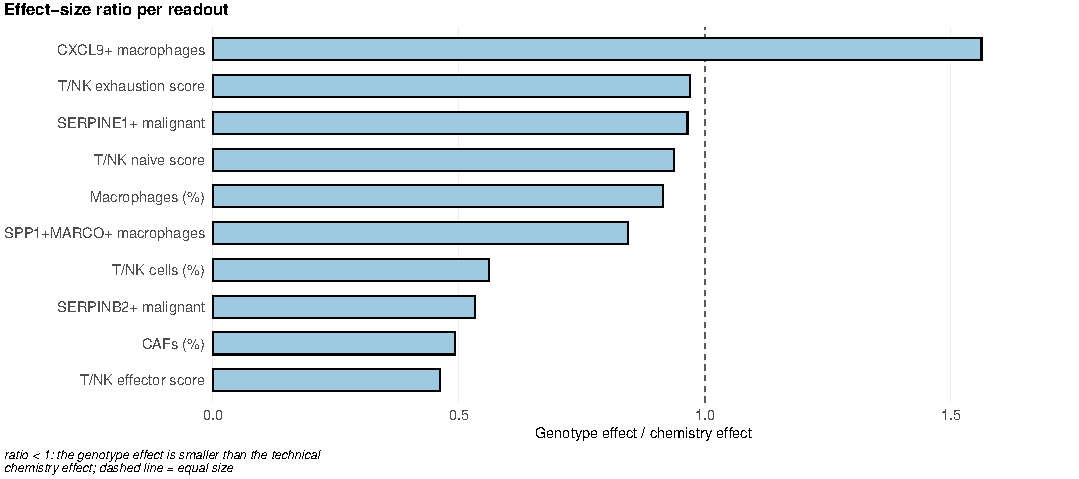
\includegraphics[width=0.95\textwidth]{figS3_effects.pdf}
\caption{\textbf{Supplementary Fig.~S3.} Genotype versus chemistry
effect sizes per readout, redrawn in R/ggplot2 as the ratio of the
two effect sizes (dashed line = parity). Nine of ten readouts fall
below parity: the chemistry effect meets or exceeds the genotype
effect, so a pooled six-library analysis would alias genotype with
chemistry. This panel is not in the source paper; it quantifies the
confound behind Table~\ref{tab:effects}.}
\label{fig:effects}
\end{figure}

%% ======================================================================
%%  REPRODUCTION SUMMARY
%% ======================================================================

\section{Reproduction summary}

Table~\ref{tab:verdicts} (Appendix, p.~\pageref{tab:verdicts})
summarises every claim testable from the public deposits, organised by
the source paper's 13 sections. It is set as a long table at the end of
the report so that it can break across pages without displacing the
figures.


\section{Discussion}

\textbf{The scRNA-seq biology is directionally reproducible, but
only within chemistry.} Every scRNA-seq claim above was scored in
the chemistry the source analysis used. In the other chemistry,
several contrasts reverse sign. The two chemistries are technical
replicates of the same three tumours, so a pooled six-library
analysis will manufacture genotype--chemistry aliases with
plausible fold changes. The source paper's own platform split
(fresh libraries for immunity, Flex for stroma) implicitly
acknowledges chemistry dominance; we make it explicit.

\textbf{The deposit cannot confirm the perturbations.} Perturb-map
tumours are mosaic; Serpine1 detection persists in the Serpine1-KO
libraries and in classic is the \emph{highest} of the three
genotypes. Knockdown validation for this deposit exists only in the
source paper's western blots (ED Fig.~5b), which are not
recomputable.

\textbf{All p-values of the non-deposited panels are confirmed.}
The in vivo, flow, IHC and survival p-values recompute to values
that match or are more conservative than the claimed numbers. One
attribution error was identified: the claimed 0.0024 in Fig.~2n
is the PAI-039-vs-combo contrast, not Vehicle-vs-PAI-039. The
3j/3l p-value set is confirmed but permuted in legend attribution.
The mixing experiment's claimed 0.0578 is the Serpine1-KO vs mix
contrast, not a Control contrast. Figure~1 (Perturb-map screen)
has no source-data file and remains a documented gap.

\section{Limitations}

\begin{enumerate}
\item \textbf{One tumour per genotype.} Every fold change in the
scRNA-seq component is a ratio of two single tumours; tumour
identity and genotype are perfectly confounded. No cell-level
p-values are reported because none would be valid.
\item \textbf{Reconstruction, not replay.} The upstream pipeline
was reconstructed from the Methods text; cell-level numbers
differ from the source's, which is why all scRNA-seq verdicts are
directional.
\item \textbf{T-cell state definitions.} Per-cell module-score
rules were used because classic-only clustering did not resolve
exhausted states; the prog, int and term tertile split is rank-based
and assigned all ``term'' cells to one library, so we interpret
only the combined Tex fraction.
\item \textbf{Platform ambiguity of Fig.~4g.} The source Methods
do not state which chemistry underlies the macrophage-state
analysis; the claims reproduce in classic and fail in Flex.
\item \textbf{Fig.~1 cannot be re-plotted.} The Perturb-map
screen (fitness heatmaps, niche-enrichment heatmaps, clone-fate
scoring) has no source-data file in the Nature supplement.
\item \textbf{Human components out of scope.} Sections 11--12
(human spatial niches, human scRNA compendium) rely on
dbGaP-controlled or separate public datasets not attempted here.
\end{enumerate}

\section*{Reporting note}

This report contains no cell-level p-values for the scRNA-seq
component. The unit of inference is the tumour (n = 1 per
genotype); all scRNA-seq quantities are per-library descriptive
fractions, signature means, or ratios thereof. Every non-deposited
panel p-value is recomputed from the Nature source-data
spreadsheets. All numbers are regenerated by
\path{methods_paper/audit_mouse_confound.py} (flag
\texttt{--source-data} for the MOESM re-plot; default for the
scRNA-seq readouts) from
\path{serpin_repro/processed/GSE289138_processed.h5ad}.

\section*{Data and code availability}

\begin{itemize}
\item Mouse scRNA-seq: GEO \texttt{GSE289138} (processed 10x
triplets; no FASTQ). Perturb-map Multi-modal raw data: Zenodo
\texttt{10.5281/zenodo.18882157}. Source code of the original
study: \path{github.com/BDBrownLab/Falcomata_PDAC_2026}
(figure-level notebooks only; open issue \#1 requests six
undistributed input files) and
\path{github.com/srose89/Perturb-map}.
\item Nature source data: \texttt{MOESM9--17} (archived in
\path{serpin_repro/data/Nature_SourceData/}); 13 xlsx files.
\item Reconstruction code: \path{serpin_repro/pdac_sc_preprocessing.py}
(genotype re-run with metadata assertions),
\path{serpin_repro/step3_annotate_cnv.py},
\path{serpin_repro/step4_myeloid.py},
\path{methods_paper/audit_mouse_confound.py} (all tables and
per-library readouts in this report; flag \texttt{--source-data} for
the legacy matplotlib MOESM re-plot), and
\path{methods_paper/figs_nature.R} (R~4.6.1 + ggplot2; regenerates
all 15 panel-for-panel composites, Figs.~1--5 and Extended Data
Figs.~1--10, plus Supplementary Figs.~S1--S3, into
\path{methods_paper/figs_nature/}).
\item Design corrections: \path{CORRECTIONS.md} C4 (fabricated
treatment column; real design 3 genotypes $\times$ 2 chemistries)
and C6 (this reproduction audit); authoritative metadata
\path{serpin_repro/processed/sample_metadata_CORRECTED.tsv}.
\end{itemize}

\begin{thebibliography}{9}

\bibitem{falcomata2026}
Falcomat\`a, C. et al. A serpin--myeloid axis in pancreatic cancer
heterogeneity and immune evasion. \emph{Nature} \textbf{658},
1330--1340 (2026). doi:10.1038/s41586-026-11002-8

\bibitem{dhainaut2022}
Dhainaut, M. et al. Spatial CRISPR genomics identifies regulators of
the tumor microenvironment. \emph{Cell} \textbf{185}, 1223--1239
(2022).

\bibitem{corrections}
Internal correction log: \path{CORRECTIONS.md}, corrections C4
and C6 (this project), 2026.

\bibitem{repo}
Open issue \#1, \texttt{BDBrownLab/Falcomata\_PDAC\_2026}: request
for six missing Perturb-map Multi-modal input files (opened
2025-10-10, unresolved).

\bibitem{zenodo}
Falcomat\`a, C. A serpin-myeloid axis in pancreatic cancer
heterogeneity and immune evasion (version v1) [Data set]. Zenodo
\texttt{10.5281/zenodo.18882157} (2026).

\end{thebibliography}


\clearpage
\section*{Extended Data figures}
\addcontentsline{toc}{section}{Extended Data figures}

Every Extended Data figure of the source paper is rebuilt panel for
panel, with the paper's own panel letters. Panels whose numbers are
in MOESM13--17 are redrawn; panels recomputable from GSE289138 are
recomputed; the remainder are grey placeholders stating why they
cannot be rebuilt from public deposits.

\begin{figure}[htbp]
\centering
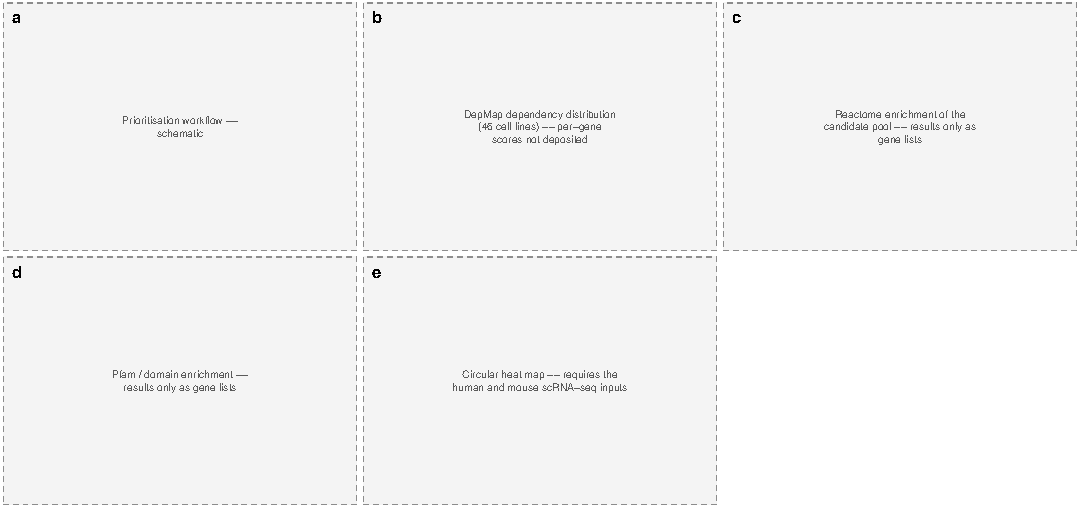
\includegraphics[width=\textwidth]{ed1.pdf}
\caption{\textbf{Extended Data Fig.~1.} All five panels are
placeholders. \textbf{a}, prioritisation workflow; \textbf{b}, DepMap
dependency distributions over 46 cell lines; \textbf{c},
Reactome enrichment; \textbf{d}, Pfam/domain enrichment; \textbf{e},
circular expression heat map. No source-data sheet exists for this
figure, and the panels are drawings or summaries whose per-gene
output was never deposited; the candidate list survives only as
Supplementary Table~1.}
\label{fig:ed1}
\end{figure}

\begin{figure}[htbp]
\centering
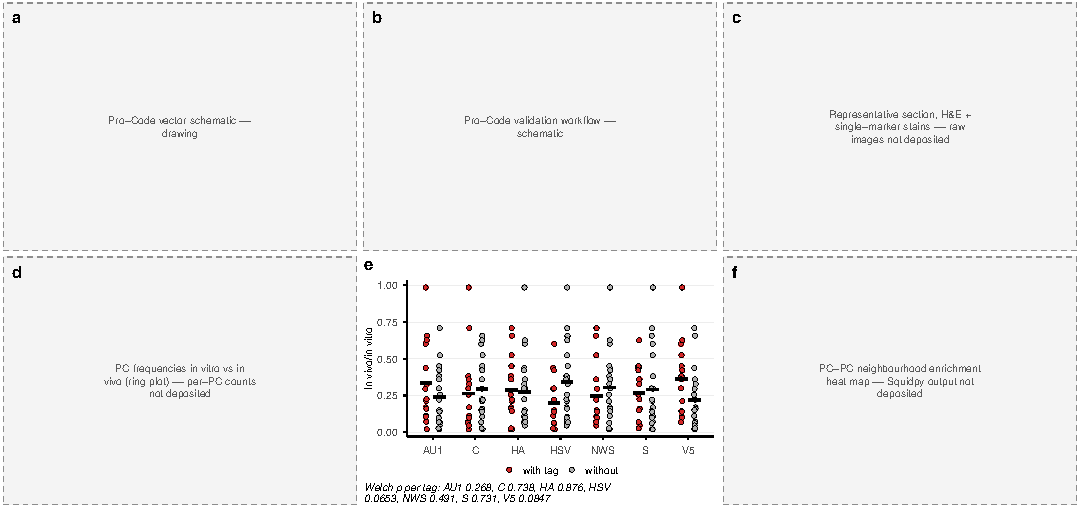
\includegraphics[width=\textwidth]{ed2.pdf}
\caption{\textbf{Extended Data Fig.~2.} \textbf{Redrawn from
MOESM13:} \textbf{e}, relative in vivo/in vitro frequency of each
Pro-Code, split by epitope tag, with the per-tag Welch $p$ recomputed
from the deposited values. \textbf{Placeholders:} \textbf{a},
\textbf{b}, vector and validation schematics; \textbf{c},
representative H\&E and single-marker sections; \textbf{d}, in vitro
versus in vivo Pro-Code frequencies (per-Pro-Code counts not
deposited); \textbf{f}, Squidpy neighbourhood-enrichment heat map.}
\label{fig:ed2}
\end{figure}

\begin{figure}[htbp]
\centering
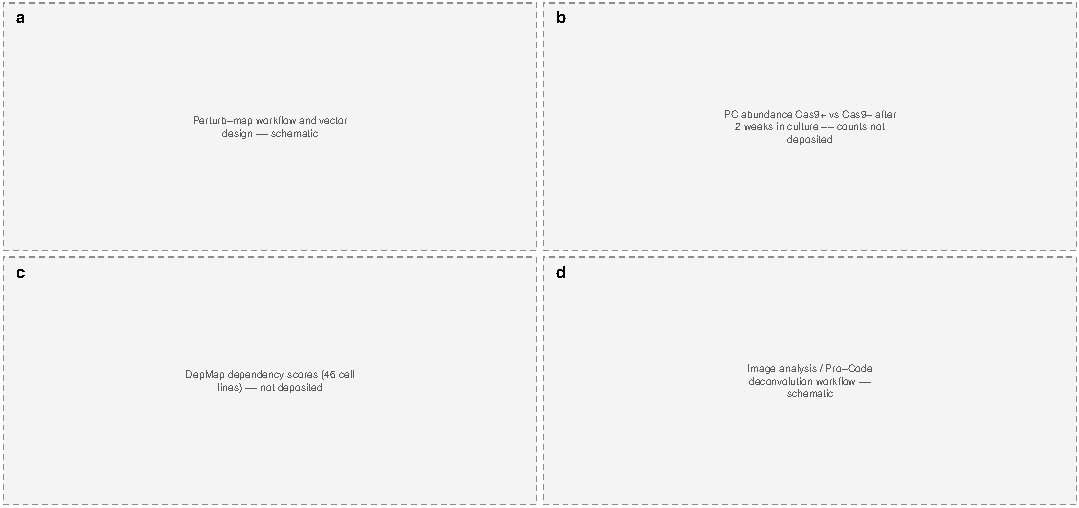
\includegraphics[width=0.92\textwidth]{ed3.pdf}
\caption{\textbf{Extended Data Fig.~3.} All four panels are
placeholders: \textbf{a}, Perturb-map workflow and vector design;
\textbf{b}, Pro-Code abundance in Cas9$^{+}$ versus Cas9$^{-}$ cells
after two weeks in culture; \textbf{c}, DepMap dependency scores;
\textbf{d}, image-analysis and Pro-Code deconvolution workflow. The
screen counts behind \textbf{b} and \textbf{c} are not deposited.}
\label{fig:ed3}
\end{figure}

\begin{figure}[htbp]
\centering
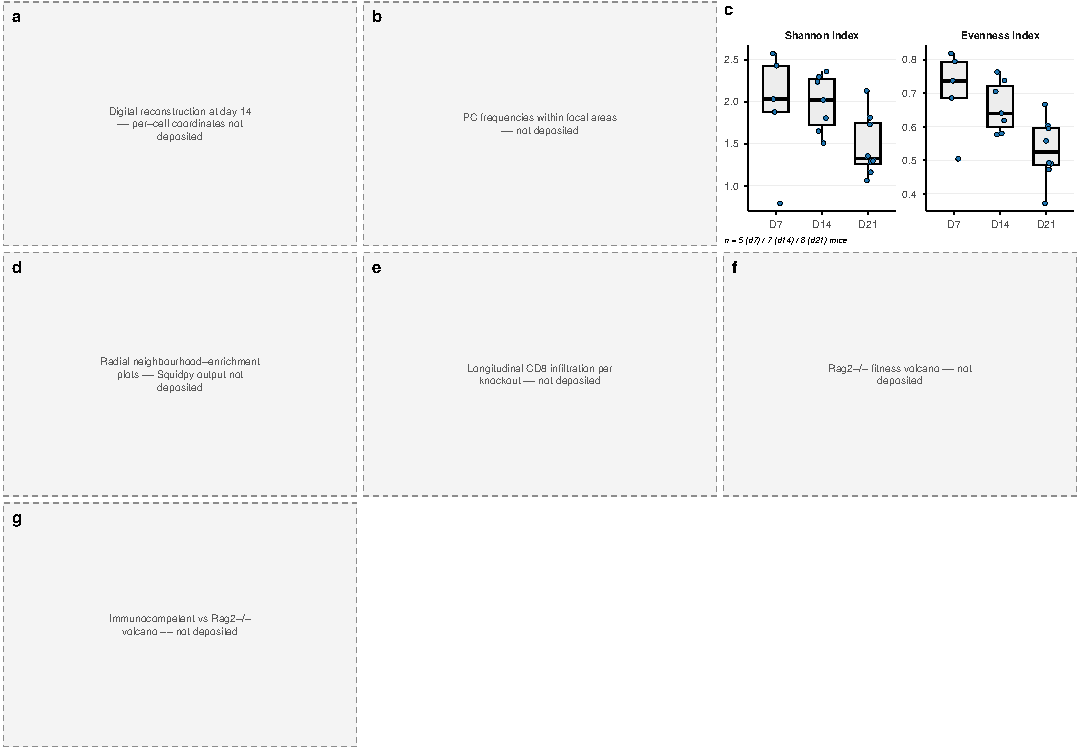
\includegraphics[width=\textwidth]{ed4.pdf}
\caption{\textbf{Extended Data Fig.~4.} \textbf{Redrawn from
MOESM14:} \textbf{c}, Shannon and Evenness indices of the Pro-Code
population at days 7, 14 and 21 (n = 5/7/8 mice), shown as
box-and-point panels. \textbf{Placeholders:} \textbf{a}, digital
reconstruction at day 14; \textbf{b}, Pro-Code frequencies within
focal areas; \textbf{d}, radial neighbourhood-enrichment plots;
\textbf{e}, longitudinal CD8 infiltration; \textbf{f}, \textbf{g},
Rag2$^{-/-}$ and immunocompetent fitness volcano plots. All require
per-cell coordinates or per-gene statistics that were not deposited.}
\label{fig:ed4}
\end{figure}

\begin{figure}[htbp]
\centering
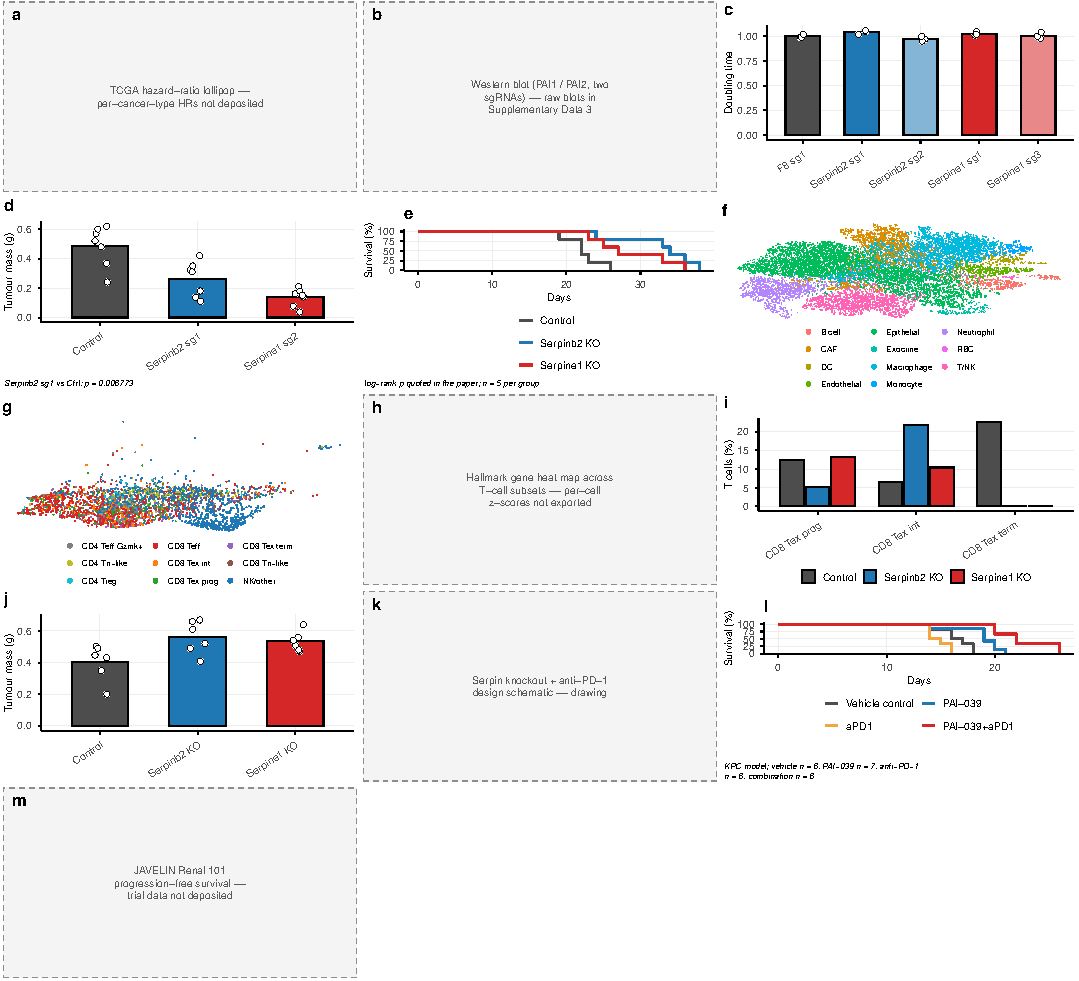
\includegraphics[width=\textwidth]{ed5.pdf}
\caption{\textbf{Extended Data Fig.~5.} \textbf{Redrawn from
MOESM15:} \textbf{c}, relative doubling time -- deposited as a ratio
normalised to $\approx$1 for every group, i.e.\ no measurable
proliferation effect of either knockout; \textbf{d}, tumour mass at
day 14 with secondary sgRNAs; \textbf{e}, survival with secondary
sgRNAs, drawn as a no-censoring Kaplan--Meier because the sheet is an
event table (5 mice per arm); \textbf{j}, tumour mass in Rag2$^{-/-}$
hosts; \textbf{l}, survival under vehicle, PAI-039, anti-PD-1 and
combination (6/7/6/6 mice). \textbf{Recomputed from GSE289138:}
\textbf{f}, UMAP of the major populations; \textbf{g}, T-cell subset
UMAP; \textbf{i}, terminally exhausted CD8 subsets. \textbf{Placeholders:}
\textbf{a}, TCGA hazard-ratio lollipop; \textbf{b}, western blot for
PAI1/PAI2 with two sgRNAs (raw blots are in Supplementary Data~3);
\textbf{h}, hallmark-gene heat map across T-cell subsets;
\textbf{k}, knockout-plus-anti-PD-1 design schematic; \textbf{m},
JAVELIN Renal 101 progression-free survival.}
\label{fig:ed5}
\end{figure}

\begin{figure}[htbp]
\centering
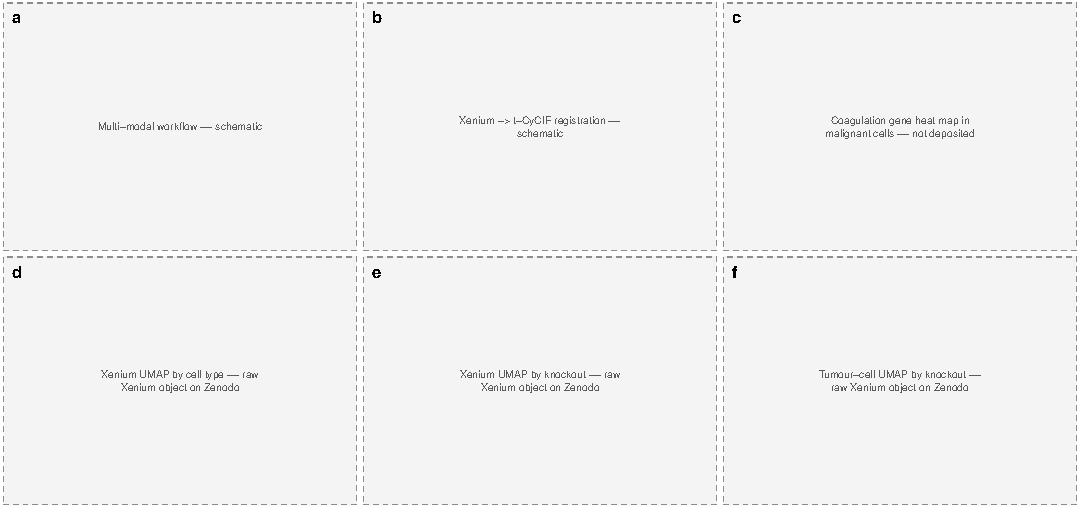
\includegraphics[width=\textwidth]{ed6.pdf}
\caption{\textbf{Extended Data Fig.~6.} All six panels are
placeholders: \textbf{a}, multi-modal workflow; \textbf{b}, Xenium to
t-CyCIF registration; \textbf{c}, coagulation-gene heat map in
malignant cells; \textbf{d}--\textbf{f}, Xenium UMAPs by cell type, by
knockout and for tumour cells. The Xenium object is on Zenodo but no
figure-level source data or processed coordinate table was deposited.}
\label{fig:ed6}
\end{figure}

\begin{figure}[htbp]
\centering
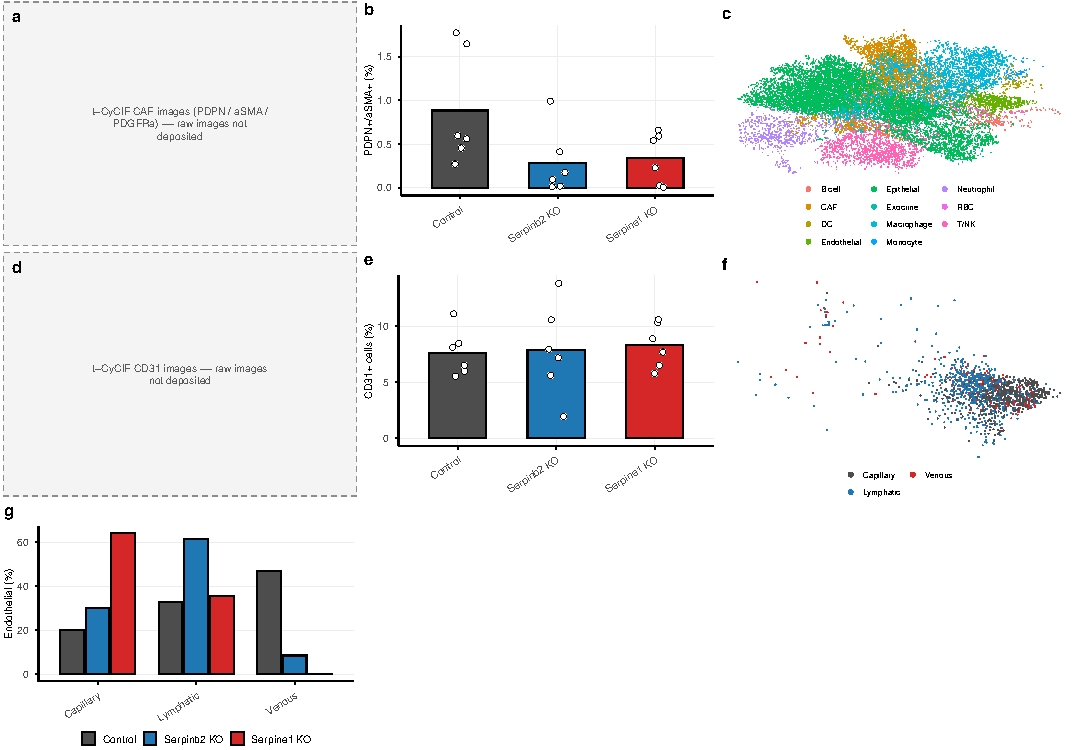
\includegraphics[width=\textwidth]{ed7.pdf}
\caption{\textbf{Extended Data Fig.~7.} \textbf{Redrawn from
MOESM16:} \textbf{b}, PDPN$^{+}$/aSMA$^{+}$ cell fraction; \textbf{e},
CD31$^{+}$ cell fraction. The deposit supplies no axis labels for
these sheets, so ordinates are arbitrary units. \textbf{Recomputed
from GSE289138 (Flex libraries):} \textbf{c}, UMAP of the major
populations; \textbf{f}, endothelial subset UMAP; \textbf{g},
endothelial subset composition (capillary, lymphatic, venous).
\textbf{Placeholders:} \textbf{a}, \textbf{d}, t-CyCIF images of CAFs
and endothelium.}
\label{fig:ed7}
\end{figure}

\begin{figure}[htbp]
\centering
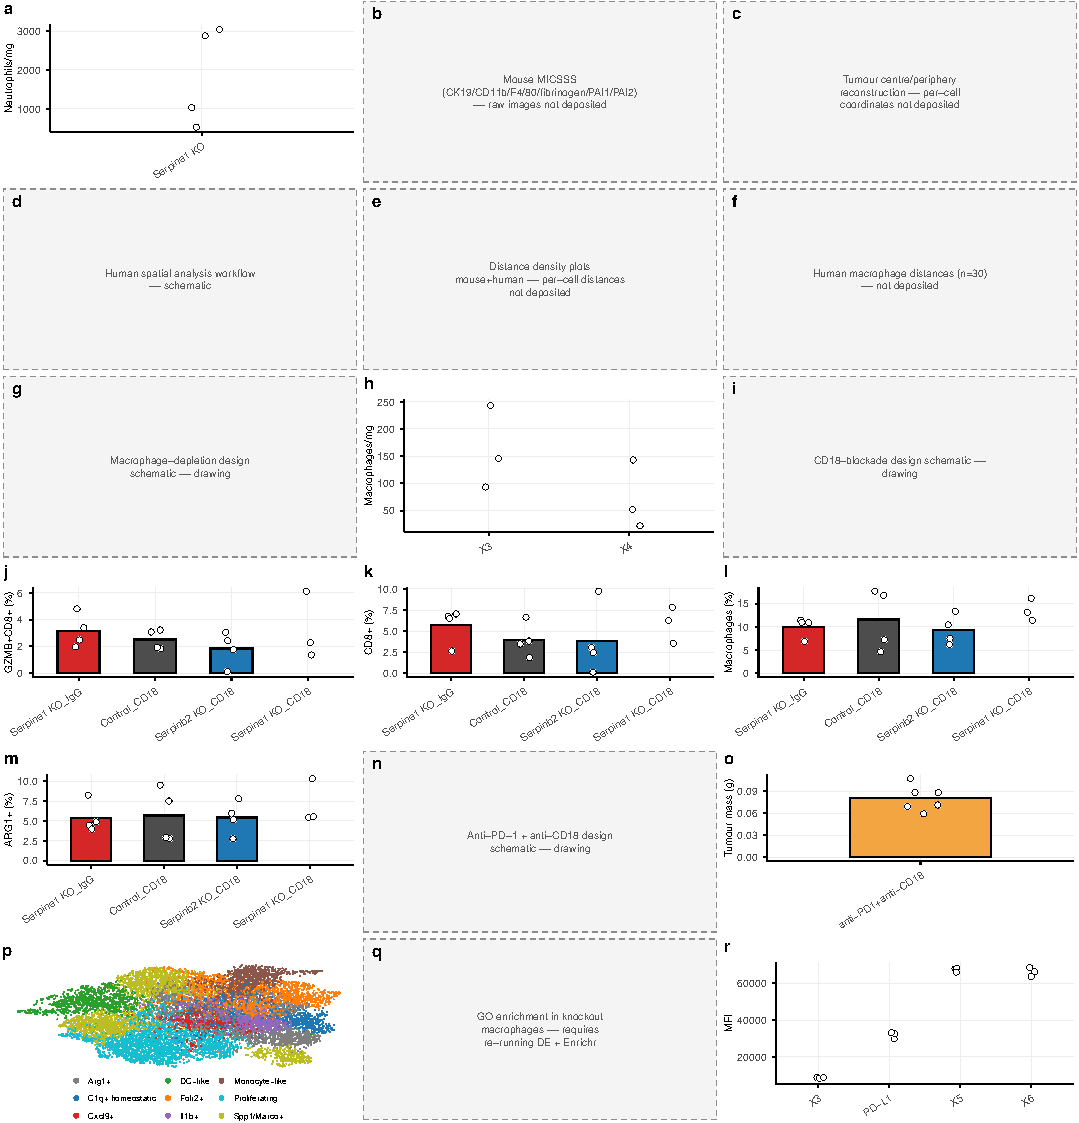
\includegraphics[width=\textwidth]{ed8.pdf}
\caption{\textbf{Extended Data Fig.~8.} \textbf{Redrawn from
MOESM17:} \textbf{a}, neutrophils per mg; \textbf{h}, macrophages per
mg; \textbf{j}, GZMB$^{+}$CD8$^{+}$ fraction; \textbf{k}, CD8$^{+}$
fraction; \textbf{l}, macrophage fraction; \textbf{m}, ARG1$^{+}$
macrophage fraction; \textbf{o}, tumour mass; \textbf{r}, MFI. Group
labels are taken from the two header rows of each sheet (merged
super-group cells carried to the right) and the light tint marks the
second level of the same genotype (e.g.\ $\pm$ anti-CSF1/clodronate,
$\pm$ aCD18); the sheets carry no axis labels, so ordinates are
arbitrary units. \textbf{Recomputed from GSE289138:} \textbf{p},
macrophage subset UMAP. \textbf{Placeholders:} \textbf{b}--\textbf{f},
mouse and human multiplex imaging, spatial reconstruction and
distance-density plots; \textbf{g}, \textbf{i}, \textbf{n}, depletion
and blockade design schematics; \textbf{q}, GO enrichment in knockout
macrophages.}
\label{fig:ed8}
\end{figure}

\begin{figure}[htbp]
\centering
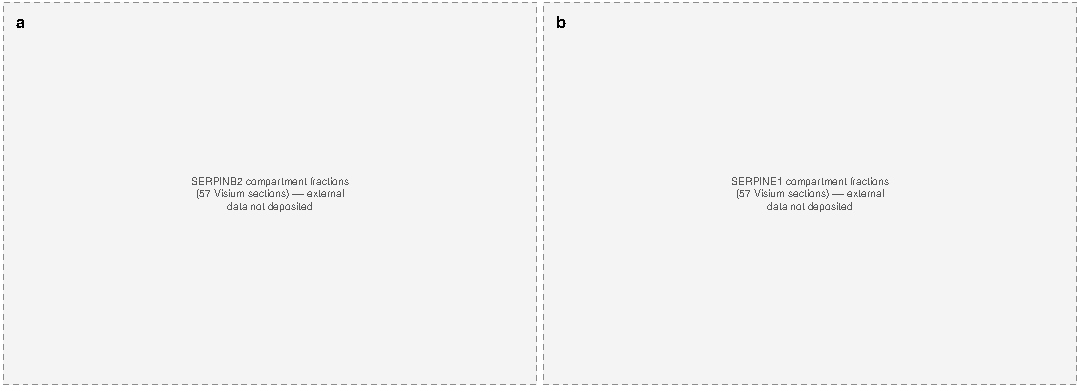
\includegraphics[width=0.86\textwidth]{ed9.pdf}
\caption{\textbf{Extended Data Fig.~9.} Both panels are placeholders:
\textbf{a}, SERPINB2 and \textbf{b}, SERPINE1 compartment fractions
across 57 Visium sections from 57 patients with stage III melanoma
treated with adjuvant anti-PD-1. The cohort is external
(GSE300793/GSE300445/446) and the per-section response mapping is
published only as a supplementary PDF, so no panel can be rebuilt
from the deposit.}
\label{fig:ed9}
\end{figure}

\begin{figure}[htbp]
\centering
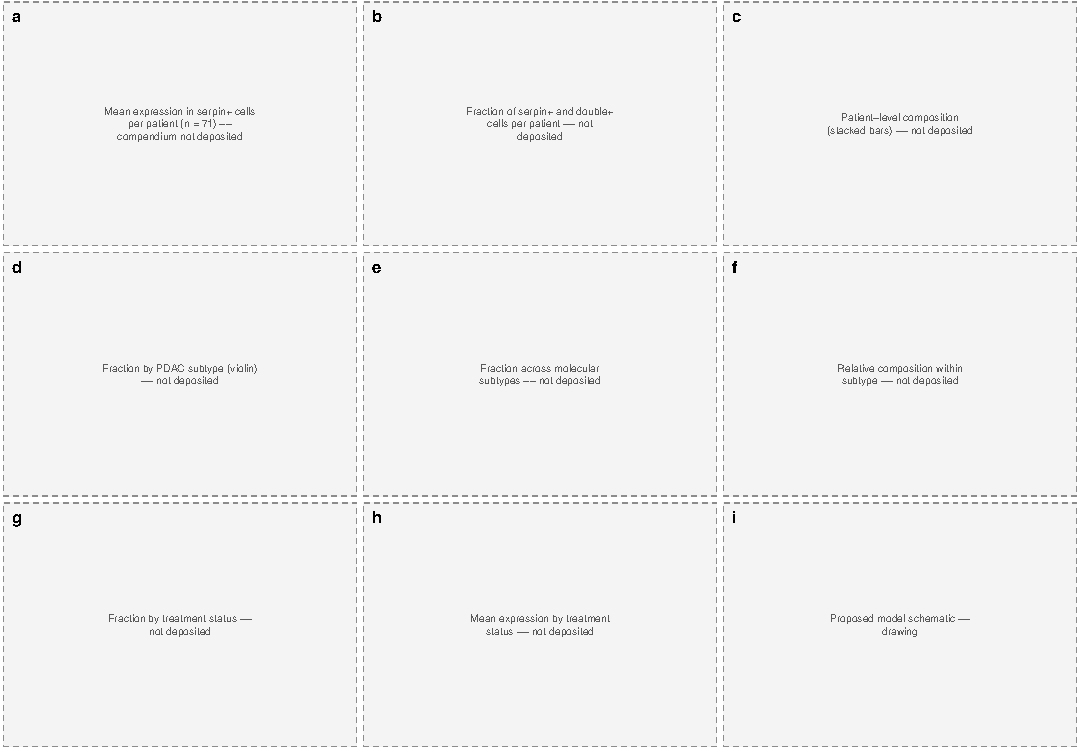
\includegraphics[width=\textwidth]{ed10.pdf}
\caption{\textbf{Extended Data Fig.~10.} All nine panels are
placeholders: \textbf{a}--\textbf{h}, per-patient mean expression,
serpin-positive and double-positive fractions, patient composition,
PDAC subtype and molecular-subtype distributions, and treatment-status
contrasts in the 71-patient human scRNA-seq compendium;
\textbf{i}, proposed model schematic. The compendium is a separate
five-dataset integration that is not deposited as a single object.}
\label{fig:ed10}
\end{figure}


\clearpage
\section*{Appendix: reproduction verdicts}
\addcontentsline{toc}{section}{Appendix: reproduction verdicts}

{\footnotesize
\renewcommand{\arraystretch}{0.94}
\setlength{\LTpre}{2pt}\setlength{\LTpost}{2pt}
\begin{longtable}{>{\raggedright\arraybackslash}p{4.6cm}>{\raggedright\arraybackslash}p{1.4cm}>{\raggedright\arraybackslash}p{5.2cm}>{\raggedright\arraybackslash}p{1.5cm}}
\caption{Reproduction verdicts. scRNA-seq claims are assessed in the
chemistry the source analysis used (classic for immunity, Flex for
stroma). Non-deposited panels are re-plotted from MOESM9--17 with
recomputed p-values. $\checkmark$ = confirmed; $\times$ = not
reproduced; $-$ = not characterisable or not re-plottable.}
\label{tab:verdicts}\\
\toprule
Source claim (section) & Source & Reproduction & Verdict \\
\midrule
\endfirsthead
\toprule
Source claim (section) & Source & Reproduction & Verdict \\
\midrule
\endhead
\bottomrule
\endlastfoot
\multicolumn{4}{l}{\textbf{\S1--4: Perturb-map screen (Fig.~1, ED 1--4)}} \\
Candidate screening (ED 1) & --- & not re-plottable & $-$ \\
Pro-Code/CRISPR screen (Fig.~1a--e) & --- & raw imaging not deposited & $-$ \\
Niche modelling (Fig.~1f) & --- & raw imaging not deposited & $-$ \\
Rag2$^{-/-}$ validation (Fig.~1g--h) & --- & no source data & $-$ \\
\midrule
\multicolumn{4}{l}{\textbf{\S5: CD8 exclusion (Fig.~2a--i; ED 5)}} \\
Tumour mass reduced (Fig.~2d) & MOESM9 &
$p$ = 0.001023/0.0002745 (claimed 0.001/0.0003) & \checkmark \\
CD8 flow increased (Fig.~2e) & MOESM9 &
3.04$\times$/4.69$\times$; $p$ = 0.02874/0.04364 & \checkmark \\
Exhausted CD8 reduced (Fig.~2f, scRNA) & GSE289138 &
Tex 41.55 $\to$ 26.97/23.70\% (1.54$\times$/1.75$\times$) & \checkmark \\
CD8 Teff increased (Fig.~2f, scRNA) & GSE289138 &
33.79 $\to$ 48.86/49.38\% (1.45$\times$/1.46$\times$) & \checkmark \\
IHC CD8/GZMB (Figs.~2h,i) & MOESM9 &
$p$ = 0.001761/0.006365/0.01945/0.041 & \checkmark \\
ED 5d secondary sgRNA mass & MOESM15 &
$p$ = 0.006773/0.000246 & \checkmark \\
\midrule
\multicolumn{4}{l}{\textbf{\S6: anti-PD-1 resistance (Fig.~2j--n; ED 5)}} \\
NSG mass (Fig.~2k) & MOESM9 &
$p$ = 0.004317/0.02754 (claimed 0.0043/0.0275; 4-digit match) & \checkmark \\
aPD1 survival (Fig.~2l) & MOESM9 &
log-rank 0.000470/0.000181 (claimed 0.0002/0.0005; smaller) & \checkmark \\
PAI-039 + aPD1 (Fig.~2n) & MOESM9 &
0.0003/0.0024/0.0143 re-mapped; 0.0024 = PAI-039 vs combo & \checkmark \\
JAVELIN PFS (ED 5m) & --- & no source data & $-$ \\
\midrule
\multicolumn{4}{l}{\textbf{\S7: transcriptomic mechanism (Fig.~3a--d)}} \\
Multi-modal pathway scoring & --- & six input files missing & $-$ \\
\midrule
\multicolumn{4}{l}{\textbf{\S8: ECM remodelling (Fig.~3e--l; ED 7)}} \\
PDPN$^{+}$ CAF (Fig.~3e) & MOESM10 &
$p$ = 0.2218/0.001995 (exact match) & \checkmark \\
aSMA+PDPN CAF (Fig.~3f) & MOESM10 &
$p$ = 0.7267/0.03591 (exact match) & \checkmark \\
CAF subtype preservation (Fig.~3g--h, scRNA) & GSE289138 &
matrix CAF 62.06 $\to$ 13.33/24.78; LRCC15$^{+}$ 0 $\to$ 1.64/22.56
& \textbf{$\times$} \\
Trichrome / fibrin (Figs.~3j,l) & MOESM10 &
p-set confirmed; 3j/3l attribution permuted in legend & \checkmark \\
Endothelial unchanged (ED 7b,e) & MOESM16 &
$p$ = 0.22/0.56 (NS; consistent with paper) & \checkmark \\
\midrule
\multicolumn{4}{l}{\textbf{\S9: TAM mediation (Fig.~4a--f; ED 8)}} \\
Macrophage flow (Fig.~4a) & MOESM11 &
$p$ = 0.02193 (claimed 0.0219; exact match) & \checkmark \\
Macrophage depletion (Fig.~4e) & MOESM11 &
$p$ = 0.0021; no additive effect with Serpin KO & \checkmark \\
CD18 blockade (Fig.~4f) & MOESM11 &
$p$ = 0.0014; mimics Serpin KO; no additive & \checkmark \\
Human multiplex IHC (Fig.~4b) & --- & not deposited & $-$ \\
ED 8a--o & MOESM17 & all recomputed; confirmed & \checkmark \\
\midrule
\multicolumn{4}{l}{\textbf{\S10: TAM state programming (Fig.~4g--j)}} \\
Spp1$^{+}$/Marco$^{+}$ reduced in Serpine1-KO (Fig.~4g, scRNA) &
GSE289138 & 12.12 $\to$ 5.57\% (2.18$\times$) & \checkmark \\
Cxcl9$^{+}$ increased (Fig.~4g, scRNA) & GSE289138 &
3.02 $\to$ 6.05/7.82\% & \checkmark \\
Proliferating reduced (Fig.~4g, scRNA) & GSE289138 &
10.89 $\to$ 5.80/6.05\% & \checkmark \\
Arg1$^{+}$ mirrors serpin loss (ED 8m, scRNA) & GSE289138 &
13.60 $\to$ 21.67/23.22\% (increases) & \textbf{$\times$} \\
BMDM fibrin culture (Fig.~4i--j) & MOESM11 &
ARG1/PD-L1 $\uparrow$, CD86 unchanged; argatroban no effect
& \checkmark \\
\midrule
\multicolumn{4}{l}{\textbf{\S11--12: human validation (Fig.~4k--l, 5a--c)}} \\
Human spatial niches (Fig.~4k--l) & --- & dbGaP controlled & $-$ \\
Human scRNA compendium (Fig.~5a--c) & --- & separate analysis & $-$ \\
\midrule
\multicolumn{4}{l}{\textbf{\S13: mixing experiment (Fig.~5d--l)}} \\
Mix tumour mass (Fig.~5e) & MOESM12 &
0.0578 = Se1-KO vs mix (0.05779) & \checkmark \\
Mix macrophages/CD8/GZMB (Figs.~5f--h) & MOESM12 &
recomputed; confirmed & \checkmark \\
ROI-level spatial (Figs.~5k--l) & MOESM12 &
recomputed; confirmed & \checkmark \\
\midrule
\multicolumn{4}{l}{\textbf{Cross-cutting}} \\
Serpine1 detection persists in KO libraries (Fig.~5a, scRNA) &
GSE289138 & 23.67\% classic; 28.44\% Flex & \checkmark (mosaic;
KD not confirmable) \\
SERPINB2$^{+}$ malignant state (Fig.~5a, scRNA) & GSE289138 &
detection 0.00--0.17\% & not characterisable \\
\end{longtable}
}

\end{document}
